% This is samplepaper.tex, a sample chapter demonstrating the
% LLNCS macro package for Springer Computer Science proceedings;
% Version 2.20 of 2017/10/04
%
\documentclass[EPiC]{easychair}
\usepackage{graphicx}
\usepackage[defaultlines=4,all]{nowidow}
\usepackage{booktabs}
\usepackage{amssymb,amsmath}
\usepackage{hyperref, subcaption}

% Used for displaying a sample figure. If possible, figure files should
% be included in EPS format.
%
% If you use the hyperref package, please uncomment the following line
% to display URLs in blue roman font according to Springer's eBook style:
% \renewcommand\UrlFont{\color{blue}\rmfamily}

\begin{document}
%
\title{Kaa: A Python Implementation of Reachable Set Computation Using Bernstein Polynomials}
%
\titlerunning{Kaa: Python Reachability Tool}
% If the paper title is too long for the running head, you can set
% an abbreviated paper title here
%
\author{Edward Kim
%\orcidID{0000-1111-2222-3333} 
\and
Parasara Sridhar Duggirala
%\orcidID{1111-2222-3333-4444}}
}
%
\authorrunning{Kim and Duggirala}
% First names are abbreviated in the running head.
% If there are more than two authors, 'et al.' is used.
%
\institute{Department of Computer Science\\
University of North Carolina at Chapel Hill\\
\email{\{ehkim,psd\}@cs.unc.edu}
%\url{http://www.springer.com/gp/computer-science/lncs} \and
%ABC Institute, Rupert-Karls-University Heidelberg, Heidelberg, Germany\\
%\email{\{abc,lncs\}@uni-heidelberg.de}
}
%
\maketitle              % typeset the header of the contribution
%
\begin{abstract}
Reachable set computation is one of the many widely-used techniques for the verification of safety properties of dynamical systems. 
%
One of the simplest algorithms for computing reachable sets for discrete nonlinear systems uses parallelotope bundles and Bernstein polynomials.
%For discrete nonlinear systems, using Bernstein polynomials and parallelotope bundles for computing reachable set have been investigated in the literature.
%One of the reachable set computation techniques that has received considerable attention uses Bernstein polynomials and parallelotope bundles.
%
In this paper, we describe Kaa, a terse Python implementation of reachable set computation which leverages the widely used symbolic package \emph{sympy}.
%
Additionally, we simplify the user interface and provide easy-to-use plotting utilities.
%
%We also provide an easy to use interfact for plotting the reachable sets.
%
We believe that our tool has pedagogical value given the simplicity of the implementation and its user-friendliness.
%
%In addition to the simplicity of the implementation, our tool, named Kaa, also achieves better performance on standard benchmarks.
\end{abstract}

% \begin{keywords}
% Nonlinear Dynamical Systems; Reachable Set Computation; Bernstein Polynomials.
% \end{keywords}
%\keywords{Nonlinear Dynamical Systems; Reachable Set Computation; Bernstein Polynomials.}

%
%
%
\section{Introduction}

Reachable set computation is one of the 
%many 
important tools %available 
for verification of safety properties of dynamical and hybrid systems.
%
A simpler and easier-to-understand reachable set computation algorithm that utilizes Bernstein polynomials and parallelotopes has been presented in~\cite{dang2009image}.
%
Several cumulative improvements~\cite{dang2012reachability,sassi2012reachability,dang2014parameter,dreossi2016parallelotope,dreossi2017reachability} have been proposed to improve its accuracy and efficiency.
%
The tool SAPO~\cite{dreossi2017sapo} which implements these algorithms in C\texttt{++} is available publicly.
%
In this paper, we present a Python implementation of algorithm presented in~\cite{dreossi2017reachability}.
%
Our motivation for reimplementing the algorithms in Python is two-fold.
%
First, using standard libraries for symbolic manipulation in Sympy, the algorithm for reachability can be implemented concisely.
%
In fact, the main algorithm for computing the reachable set has be implemented in only one file with $150$ lines of code.
%
The total code base for Kaa is roughly only $650$ lines of code.
%
%Additionally, the main algorithm for computing the reachable set is provided in just one file with $150$ lines of code.
%
In contrast, SAPO consists of more than $2000$ lines of C\texttt{++} code with memory and pointer management performed completely by the developer.
%
We believe that such a simple implementation can be used for teaching one of the main algorithms for reachability of nonlinear systems.
%
% Second, because of its implementation in C++, SAPO requires recompiling the code for every reachable set computation.
% %
Second, reimplementing the tool in Python makes user interaction significantly simpler. 
%
In SAPO, one has to recompile the code along with the model file to generate the binary. Subsequently the user has to execute the binary to compute the reachable set.
%
Additionally, visualizing the reachable set using SAPO is a two step process. In the first step, SAPO generates a MATLAB script which plots projections of reachable set for visualizing time or phase plots of the reachable set. In the second step, the user feeds the generated script into either MATLAB or GNU Octave to illustrate the reachable set. 
%
In contrast, Kaa offers plotting functionalities through the \emph{matplotlib} library for visualizing the reachable set.
%
The models and the code for computing reachable set using Kaa are provided in Python and do not require any compilation steps.
%
Integrating these two, we provide an easy-to-use Jupyter notebook interface for computing and visualizing reachable set with Kaa for some of the standard benchmark models.
%
%Juypter notebooks are simple to create and known for their straightforward user interface. %
%we were able to design an engaging interactive tutorial and experimentation platform for visualzing reachable sets of non-linear systems.
%
%Therefore, the user has to 
%we believe that for reimplementing it in Python improves the quality of user interaction with the tool and removes the barrier to use the tools.
%

Bernstein polynomials are also an active area of research in the domain of global optimization~\cite{nataray2002algorithm,garloff2003bernstein,nataraj2007new}.
%
Several heuristics have been proposed for improving the performance of optimization using Bernstein polynomials~\cite{kodiak,smith2009fast,munoz2013formalization}. 
%
%Furthermore, these algorithms also improve the accuracy using sequential refinement techniques~\cite{}.
%
Having an accessible and flexible tool would make it more conducive to implement these heuristics and determine if they are helpful in the domain of reachability.
%
In light of these features and advantages, we believe Kaa could be used as a natural first step for introducing reachability in a pedagogical setting.

\section{Preliminaries}

The state of a system, denoted as $x$, lies in a domain $D \subseteq \mathbb{R}^n$. A discrete-time polynomial nonlinear system is denoted as

\begin{equation}
    x^{+} = f(x)
\label{eq:system}
\end{equation}
where $f(x) : \mathbb{R}^n \rightarrow \mathbb{R}^n$ is polynomial in $x$. 
%
The trajectory of the system that evolves according to Equation~\eqref{eq:system}, denoted as $\xi(x_0)$, is the sequence $x_0, x_1, \ldots$ where $x_{i+1} = f(x_i)$. 
%
The $k^{th}$ element in this sequence is denoted as $x_k = \xi(x_0,k)$.
%
Given an initial set $\Theta$, the reachable set at time $k$, denoted as $\Theta_{k} = \{~ \xi(x_0,k)~|~ x_0 \in \Theta\}$.

A parallelotope $P$ is a set of states in $\mathbb{R}^{n}$ denoted as $\langle \Lambda, c\rangle$ where $\Lambda \in \mathbb{R}^{2n \times n}$ and $c \in \mathbb{R}^{2n}$, $\Lambda_{i+n} = -\Lambda_{i}$ and $i \in \{1, \ldots, n\}$ such that

$$
x \in P \mbox{ if and only if } \Lambda x \leq c.
$$
$\Lambda$ is called the \emph{direction matrix} $\Lambda_i$ denotes the $i^{th}$ row of $\Lambda$. $c$ is called the \emph{offset}. 
%
Alternatively, a parallelotope can also be represented in vertex-generator representation as $\langle v, g_1, \ldots, g_n\rangle$. Here $v \in \mathbb{R}^n$ is called vertex and $g_1, \ldots, g_n$, $g_i \in \mathbb{R}^n$, are called generators. The parallelotope is defined as
$$
P \triangleq \{ x ~|~ \exists \alpha_1, \ldots, \alpha_n, x = v + \alpha_1 g_1 + \ldots + \alpha_n g_n, 0 \leq \alpha_i \leq 1\}
$$
This representation is very similar to Zonotopes~\cite{girard2005reachability,althoff2010computing} and Star sets~\cite{duggirala2016parsimonious}. 
%
Notice that for a parallelotope $P$, the vertex-generator representation also defines the affine transformation that maps $[0,1]^{n}$ to $P$. 
%
We denote this affine transformation as $T_{p}$. 
%
A parallelotope bundle $Q$ is a set of parallelotopes $\{P_1, \ldots, P_m\}$ where $Q = \cap_{i=1}^{m}P_i$.

Given two multi-indices $i$ and $d$ of size $n$, where $i \leq d$, the Bernstein polynomial of degree $d$ and index $i$ is 
$$
\mathcal{B}_{i,d} = \beta_{i_1,d_1}(x_1) \beta_{i_2,d_2}(x_2)\ldots \beta_{i_n,d_n}(x_n).
$$
%
where $\beta_{i_m,d_m}(x_m) = \binom{d_m}{i_m}x_{m}^{i_m}(1-x_m)^{d_m - i_m}$. 
%
Any polynomial function can be expressed in the Bernstein basis. 
%
The primary advantage of the Bernstein representation of a polynomial $h(x_1,...,x_n)$ is that an upper bound on the supremum and lower bound on the infimum of $h(x_1,...,x_n)$ in $[0,1]^{n}$ can be computed purely by observing the coefficients of the polynomial in the Bernstein basis.

In other words, given a polynomial $h(x_1,\ldots,x_n) = \sum_{j \in J} a_j {\bf x}_{j}$ where $J$ is a set of multi-indices iterating through the degrees found in $p$ with $a_j \in \mathbb{R}$, then $h(x_1,\ldots,x_n)$ can be converted into its counterpart under the Bernstein basis, $h(x_1,\ldots,x_n) = \sum_{j \in J} b_j \mathcal{B}_j $ where $b_j$ are the corresponding Bernstein coefficients. 
%
The upper and lower bounds of $h(x_1,\ldots,x_n)$ over $[0,1]^n$ are bounded by the Bernstein coefficients:
$$
min \{b_1, \ldots, b_m\} ~~\leq~~ inf_{x \in [0,1]^n} h(x) ~~~~~\leq~~~~ sup_{x \in [0,1]^{n}} h(x) ~~\leq~~ max \{b, \ldots, b_m\}.
$$

As mentioned earlier, a parallelotope $P$ can also be represented as an affine transformation $T_{p}$ from $[0,1]^{n}$ to $P$. 
%
Therefore, upper bounds on the suprenum of a function $h$ over $P$ is equivalent to upper bound of $h \circ T_{p}$ over $[0,1]^{n}$.
%
A similar argument follows for the lower bound on the infimum.
%

For the remainder of the document, we assume that by using functional composition and the Bernstein representation, we can compute the upper bound on supremum and the lower bound on the infimum of polynomial functions over parallelotopes.
%
We denote the procedures for calculating such upper and lower bounds for a polynomial $h$ over some parallelotope $P$ as $\mathsf{BernsteinUpper}(h,P)$ and $\mathsf{BernsteinLower}(h,P)$ respectively. 

\section{Reachability of Nonlinear Systems Using Parallelotope Bundles and Bernstein Polynomials}

Given a set represented as a parallelotope bundle $Q = \{P_1, P_2, \ldots, P_m\}$ and a discrete dynamical system $x^{+} = f(x)$, we now present the method for computing an overapproximation of the image $f(Q)$ as a new parallelotope bundle $Q' = \{P_1', P_2', \ldots, P_m'\}$.
%
We ensure that direction matrix of $P_i'$ is same as $P_i$ and the computation is required only to compute the offsets. 
%
Let us denote the $j^{th}$ offset of $P_i$ and $P_i'$ as $c_{j,i}$ and $c'_{j,i}$ respectively and the $j^{th}$ direction in $P_i$ (same as $P_i'$) as $\Lambda_{j,i}$.
%
Therefore, given $\Lambda$, transformation $f$, and offsets $c_{j,i}$ for $P_i$, we have to compute the values of $c'_{j,i}$.

%
%Let us denote the $j^{th}$ offset in $P_i'$ and $c'_{j,i}$ and the direction be $\Lambda_{j,i}$.
%
If $j \leq n$, any offset $c'_{j,i}$ such that $\forall_{x\in Q} \Lambda_{j,i} \cdot f(x) \leq c'_{j,i}$ is valid.
%
%For any valid $c'_{j,i}$, it should be the case that, if $j \leq n$ $ \forall_{x \in Q} \Lambda_{j,i} \cdot f(x) \leq c'_{j,i}$.
%
If $j > n$, then any offset $c'_{j,i}$ such that $\forall_{x \in Q} \Lambda_{j-n,i} \cdot f(x) \geq c'_{j,i}$ is valid.
%
Therefore, one can compute the $j^{th}$ offset of $P_i'$, i.e., $c'_{j,i}$ for $j \leq n$ by computing an upper bound of the function $\Lambda_{j,i} \cdot f(x)$ over the $x\in P_i$.
%The algorithm for computing the $j^{th}$ offset ($j \leq n$) for $P'_i$ is the following: iterature over all the parallelotopes in the bundle and compute the upper bounds of $\Lambda_{j,i} \cdot f(x)$ over each parallotope. 
%
Similarly, the $j+n^{th}$ offset can be computed from a lower bound of the function $\Lambda_{j,i} \cdot f(x)$ over each parallelotope $x\in P_i$.
%
This is given in Equations~\ref{eq:upper} and~\ref{eq:lower}.
% Sridhar here; I am done with changes.
% Sent you an email with specific directions for submission.
% Submit the paper and let's see what they say.

\begin{eqnarray}
c_{j,i} &=& min_{l = 1}^{m} \Big\{ \mathsf{BernsteinUpper}\big(\Lambda_{j,i} \cdot f(x), P_l \big) \Big\} \mbox{ if } j \leq n. \label{eq:upper} \\
c_{j+n,i} &=& max_{l = 1}^{m} \Big\{ \mathsf{BernsteinLower}\big(\Lambda_{j,i} \cdot f(x), P_l \big) \Big\} \mbox{ otherwise. } \label{eq:lower}
\end{eqnarray}

\subsection{Python Implementation of Reachable Set Computation}

One of the primary reasons for preferring Python as the implementation language for this algorithm is the presence of powerful, well-tested symbolic and matrix-computation libraries.
%
Python's \emph{numpy} libraries are popular matrix-computation libraries which allow higher-level manipulation of matrices. This gives us an avenue of overcoming the verbosity and the possibility of memory leaks inherent in implementing identical features in C++. We believe that overcoming these obstacles results in a more readable, more compact approach to parallelotope reachability suitable for graduate students and curious practitioners. In addition, these libraries are known for their extensive set of useful functionalities which allow us to avoid reimplementing many fundamental operations.

%
As we have seen before, there are two main sub-routines for computing the reachable set using Bernstein polynomials.
%
First, performing functional composition for computing the upper bound of a polynomial over a parallelotope.
%
Second, computing the Bernstein representation of a polynomial.
%
The library of \emph{sympy} has powerful symbolic manipulation tools which allow us to comfortably perform many sensitive symbolic function composition of polynomials.
%
We use \emph{sympy}'s internal representation of polynomials to (a) perform functional composition and (b) compute the Bernstein representations of the resulting polynomial.
%
Additionally, the \emph{matplotlib} library has accessible plotting facilities that we integrate into our tool for visualizing the reachable set. In particular, \emph{matplotlib} facilitates the ability to plot several reachable sets simultaneously. This will aid others in performing more complex bundle-transformation experiments in the future. 

%
Finally, Python contains a rich set of multiprocessing libraries, namely \emph{multiprocessing} or \emph{mp} for short. We plan to exploit the parallelizable nature of bundle-transformtion computations using \emph{mp}'s ability to provide powerful multiprocessing features without much verbosity.

% c_{j+n,i} &=& max_{l = 1}^{m} \big{ \mathsf{BernsteinLower} \Lambda_{j,i}\cdot f(x) \mbox{ over } P_l \big} \mbox{ otherwsie. } \label{eq:upper}


% \subsection{A Subsection Sample}
% Please note that the first paragraph of a section or subsection is
% not indented. The first paragraph that follows a table, figure,
% equation etc. does not need an indent, either.

% Subsequent paragraphs, however, are indented.

% \subsubsection{Sample Heading (Third Level)} Only two levels of
% headings should be numbered. Lower level headings remain unnumbered;
% they are formatted as run-in headings.

\section{Evaluations}
We evaluate our tool on the benchmarks that are shipped along with SAPO. With each benchmark, the reachable sets of SAPO are juxtaposed with that of Kaa's to demonstrate the accuracy and quality of our reachable sets. A comparison of time taken by Kaa and SAPO for each benchmark is provided in Table~\ref{tab:one}.

\subsection{SIR Epidemic Model}
\noindent The SIR Epidemic model is a 3-dimensional dynamical system governed by the following dynamics:
\begin{align} \label{eqn:sir}
    \begin{split}
        s_{k+1} &= s_k - (\beta s_k i_k)\Delta \\
        i_{k+1} &= i_k + (\beta s_k i_k - \gamma i_k)\Delta \\
        r_{k+1} &= r_k + (\gamma i_k)\Delta
    \end{split}
\end{align} 
where $s,i,r$ represent the fractions of a population of individuals designated as \textit{susceptible}, \textit{infected}, and \textit{recovered} respectively. There are two parameters, namely $\beta$ and $\gamma$, which influence the evolution of the system. $\beta$ is labeled as the contraction rate and $1/\gamma$ is mean infective period. Finally, $\Delta$ is simply the discretization step. For the benchmarks, we set $\beta = 0.34$, $\gamma=0.05$, and $\Delta=0.5$. The reachable sets are displayed in Figure \ref{fig1}. The table of numerical value comparisions between Sapo and Kaa is shown in Table \ref{val1}.


\begin{table}[h]
\centering
\begin{tabular}{|c| c c c c|}
    \hline
    {\bf Time Steps} & {\bf Kaa (offu) }  & { \bf Sapo (offu) } & {\bf Kaa (offl)} & {\bf Kaa (offl) }  \\
    \hline
     50 & 0.470716 & 0.470716 & -0.435191 & -0.43519 \\
  
     51 & 0.475839 & 0.475839 & -0.439599 & -0.439599 \\ 

     52 & 0.480906 & 0.480906 & -0.443945 & -0.443945\\

     53 & 0.485915 &  0.485915 & -0.448227 &  -0.448227 \\ 

     54 & 0.490862 & 0.490862 & -0.452443 & -0.452443 \\ 

     55 & 0.495747 & 0.495747 & -0.456591 & -0.456591 \\

     56 & 0.500566 & 0.500566 & -0.460669 & -0.460669 \\ 

     57 & 0.505317 & 0.505317 & -0.464675 & -0.464675\\ 

     58 & 0.509999 & 0.509999  & -0.4686075 & -0.468608 \\ 

     59 & 0.514610 & 0.514610 & -0.472465 & -0.472465\\

     60 & 0.519147 & 0.519147 & -0.476246 & -0.476246 \\
    \hline
\end{tabular}
\caption{Comparision of offu, offl values along variable $i$ for the SIR model. We select the steps 50-60}
\label{val1}
\end{table}
\noindent Here, offu is the vector of upper offsets of the parallelotope and offl is the vector for the lower offsets. We define the upper facets of parallelotope $P$ as the $c_i$ for $i \leq n$ where $n$ is the dimension of the system and $P = \langle \Lambda, c \rangle$ is the parallelotope. Similarly, the lower facets are defined as the $c_{i+n}$ for $i \leq n$. In the case above, we are looking at values in $c_2$ and $c_{2+3} = c_5$.

\subsection{Rossler Model}
\noindent The Rossler model is another 3-dimensional system governed under the dynamics:
\begin{align} \label{rossler}
    \begin{split}
        x_{k+1} &= x_k + -(y-z)\Delta \\
        y_{k+1} &= y_k + (x_k + ay_k)\Delta \\
        z_{k+1} &= z_k + (b + z_k(x_k - c))\Delta
    \end{split}
\end{align}
where $a,b,c$ are parameters which we set to $a = 0,1$, $b =0.1$, and $c = 14$. We set our discretization step to be $\Delta= 0.025$.
The reachable sets are displayed in Figure \ref{fig2} and the table showing the comparisions between the numerical values are shown in Table \ref{val2}.

% Sridhar here: I think just giving two of these tables should be fine. No need to give tables for all of them.
% Also, there is one figure missing for KAA. Do you plan to add that?
% One thing to do is to do a screen capture of the image and upload the screen capture. Supremely hacky!
% Cool.
% Will do. Thanks.
% Yes. One figure fails to upload to Overleaf for some reason. I have to find an alternative way to upload to Overlead somehow.
% Good point. I'll look into it once I finish this table here.

\begin{table}[hbt!]
\centering
\begin{tabular}{|c| c c c c|}
    \hline
    {\bf Time Steps } & {\bf Kaa (offu) } & {\bf Sapo (offu) } & {\bf Kaa (offl) } & {\bf Kaa (offl) }  \\
    \hline
    50 & 1.95908 & 1.96043  & -1.9209 & -1.9193 \\

    51 & 1.83552 & 1.83688  & -1.7963 & -1.7947 \\
    
    52 & 1.71044 & 1.71181  & -1.67016 & -1.6685 \\
  
    53 & 1.58392 & 1.58531  & -1.54255 & -1.5409 \\
   
    54 & 1.45604 & 1.45744  & -1.41355 & -1.4119 \\
 
    55 & 1.32687 & 1.32829  & -1.28324 & -1.2815\\

    56 & 1.19649 & 1.19792  & -1.15168 & -1.1500\\

    57 & 1.06499 & 1.06642  & -1.01896 & -1.0172 \\
 
    58 & 0.932432 & 0.933877 & -0.885157 & -0.88339 \\
    
    59 & 0.798905 & 0.800358  & -0.75035 &  -0.74857 \\
  
    60 & 0.664489 & 0.665949  & -0.614619 & -0.61282\\
    \hline
\end{tabular}
\caption{Comparision of offu, offl values along variable $y$ for the Rossler model. We select the steps 50-60}
\label{val2}
\end{table}

\subsection{Quadcopter Model}
\noindent The Quadcopter model is a 17-dimensional dynamical system with the following variables:
A set of inertial positions: $(p_n,p_e,h)$, linear velocities $(u,v,w)$, the quaternions expressing the Euler angles $(q_0,q_1,q_2,q_3)$, the angular velocities $(p,q,r)$, and finally the parameters $(h_I, u_I, v_I, \psi_I)$. The complete set of dynamics and relevant parameters is found in~\cite{dreossi2017reachability} and reachable sets are shown in Figure \ref{fig3}.

% Sridhar: I added the figures, it wasn't that much effort.
% I see. Thank you.

\subsection{Lotka-Volterra Model}
\noindent We also test on the competetitive Lotka-Volterra models for predator-prey biological systems. Our instance is a 5-dimensional system governed as below:
\begin{align}
    \begin{split}
        x_{k+1} &= x_k + (x_k(1 - (x_k + \alpha y_k + \beta \ell_k))) \Delta \\
        y_{k+1} &= y_k + (y_k(1 - (y_k + \alpha z_k + \beta x_k))) \Delta \\
        z_{k+1} &= z_k + (z_k(1 - (z_k + \alpha h_k + \beta y_k))) \Delta \\
        h_{k+1} &= h_k + (h_k(1 - (h_k + \alpha \ell_k + \beta z_k))) \Delta \\
        \ell_{k+1} &= \ell_k + (\ell_k(1 - (\ell_k + \alpha x_k + \beta h_k))) \Delta
    \end{split}
\end{align}
where $\alpha,\beta$ are parameters set to $\alpha=0.85$ and $\beta=0.5$. We set $\Delta = 0.01$.
The relevant reachable sets are shown in Figure \ref{fig4}.

\subsection{Phosphoraley Model}
The Phosphoraley model describes a certain cellular regulatory system. It is captured by seven variables governed by the following dynamics:
\begin{align}
    \begin{split}
        x^1_{k+1} &= x^1_k + ( -\alpha x^1_k + \beta x^3_k x^4_k)\Delta \\
        x^2_{k+1} &= x^2_k + (  \alpha x^1_k - x^2_k)\Delta \\
        x^3_{k+1} &= x^3_k + ( x^2_k \beta x^3_k x^4_k)\Delta \\
        x^4_{k+1} &= x^4_k + ( \beta x^5_k x^6_k - \beta x^3_k x^4_k)\Delta \\
        x^5_{k+1} &= x^5_k + ( -\beta x^5_k x^6_k + \beta x^3_k x^4_k)\Delta \\
        x^6_{k+1} &= x^6_k + ( \alpha x^7_k - \beta x^5_k x^6_k)\Delta \\
        x^7_{k+1} &= x^7_k + ( -\alpha x^7_k + \beta x^5_k x^6_k)\Delta
    \end{split}
\end{align}
where $\alpha,\beta$ are two parameters assigned as $\alpha=0.5$ and $\beta=5$. We set $\Delta =0.01$ here. The figures can be found in Figure \ref{fig5}.

\subsection{Times}

\noindent It is evident from Table~\ref{tab:one} that while the current implementation in Python is intuitive and concise, it incurs severe performance penalties. 
%
Nevertheless, we pursued this direction because of the pedagogical value in making this an accessible tool for implementing and understanding reachability. To this end, the repository contains a Jupyter notebook with the name \href{https://github.com/Tarheel-Formal-Methods/kaa/blob/master/kaa-intro.ipynb}{kaa-intro} designed to interactively introduce graduate students and practitioners to the usage of Kaa. The notebook even contains a subset of the examples shown above, giving the auidence a hands-on method to run the code for themselves. An immediate next step is to deploy extensive profiling to find performance bottlenecks and subsequently improve on them. 

\begin{table}[h]
\centering
\caption{Reachable Set Computation Time of Benchmarks}\label{tab:one}
\begin{tabular}{|l | c c|}
\hline
{\bf Model} &{\bf Kaa } & {\bf SAPO } (C\texttt{++})\\
\hline
SIR &  11.41 sec & 0.16 sec\\

Rossler &  41.92 sec & 1.17 sec\\

Quadcopter & 78.21 sec & 11.98 sec \\

Lotka-Volterra & 18 min 95.05 sec  & 57.48 sec\\
 
 Phosphoraley & 103.81 sec & 24.86 sec \\
\hline
\end{tabular}
\end{table}

\section{Conclusions}

We present Kaa, a Python implementation of reachable set computation of nonlinear systems which is focused towards accessibility and pedagogical use.
%
The usage of inbuilt \emph{sympy} libraries makes the implementation short and simple (only 650 LOC).
%
While we do incur performance drawbacks from selecting Python for implementing this algorithm, we believe that it aids in fast prototyping and enables students to easily build on top of the library. In particular, Python's readability and extendibility will allow curious students to experiment with more involved bundle-transformations. 
%
The code can be accessed through \url{https://github.com/Tarheel-Formal-Methods/kaa}.
\newline
\newline
{\bf Acknowledgements: } This material is based upon work supported by the Air Force Office of Scientific Research under award number FA9550-19-1-0288 and National Science Foundation (NSF) under grant numbers CNS 1739936, 1935724. Any opinions, findings, and conclusions or recommendations expressed in this material are those of the author(s) and do not necessarily reflect the views of the United States Air Force or National Science Foundation. 

\bibliographystyle{splncs04}
\bibliography{archbib}
\newpage

\begin{figure}[h]
%    \hspace{-15ex}
    \begin{subfigure}{0.47\textwidth}
    \centering
    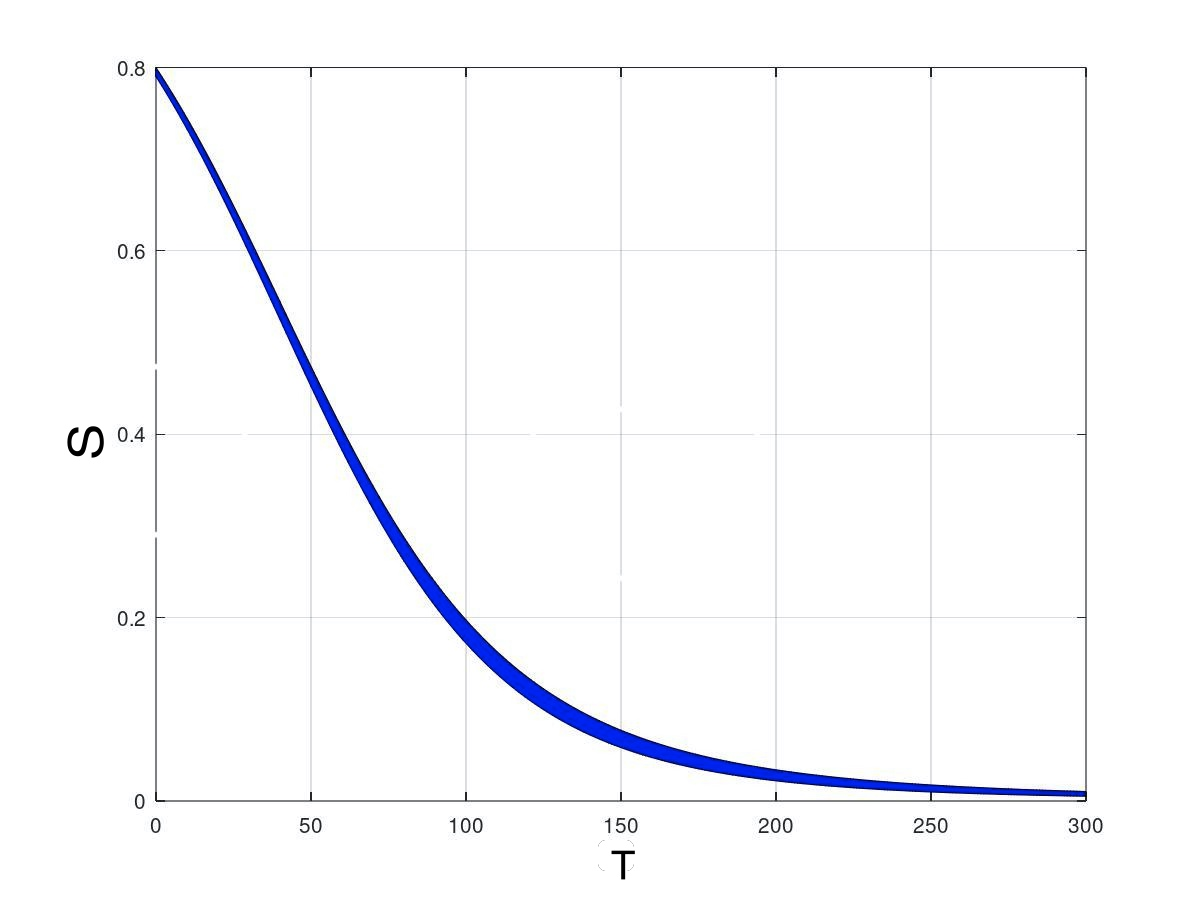
\includegraphics[width=\textwidth]{SapoFigures/SIR/SapoSIR_S.jpg}
    \end{subfigure}
    \begin{subfigure}{0.47\textwidth}
    \centering
    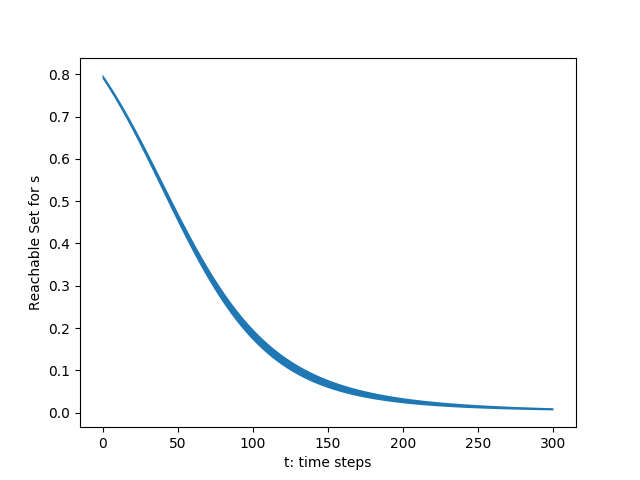
\includegraphics[width=1.2\textwidth]{SapoFigures/SIR/KaaSIR_S.png}
    \end{subfigure}
 
%    \hspace{-15ex}   
    \begin{subfigure}{0.47\textwidth}
    \centering
    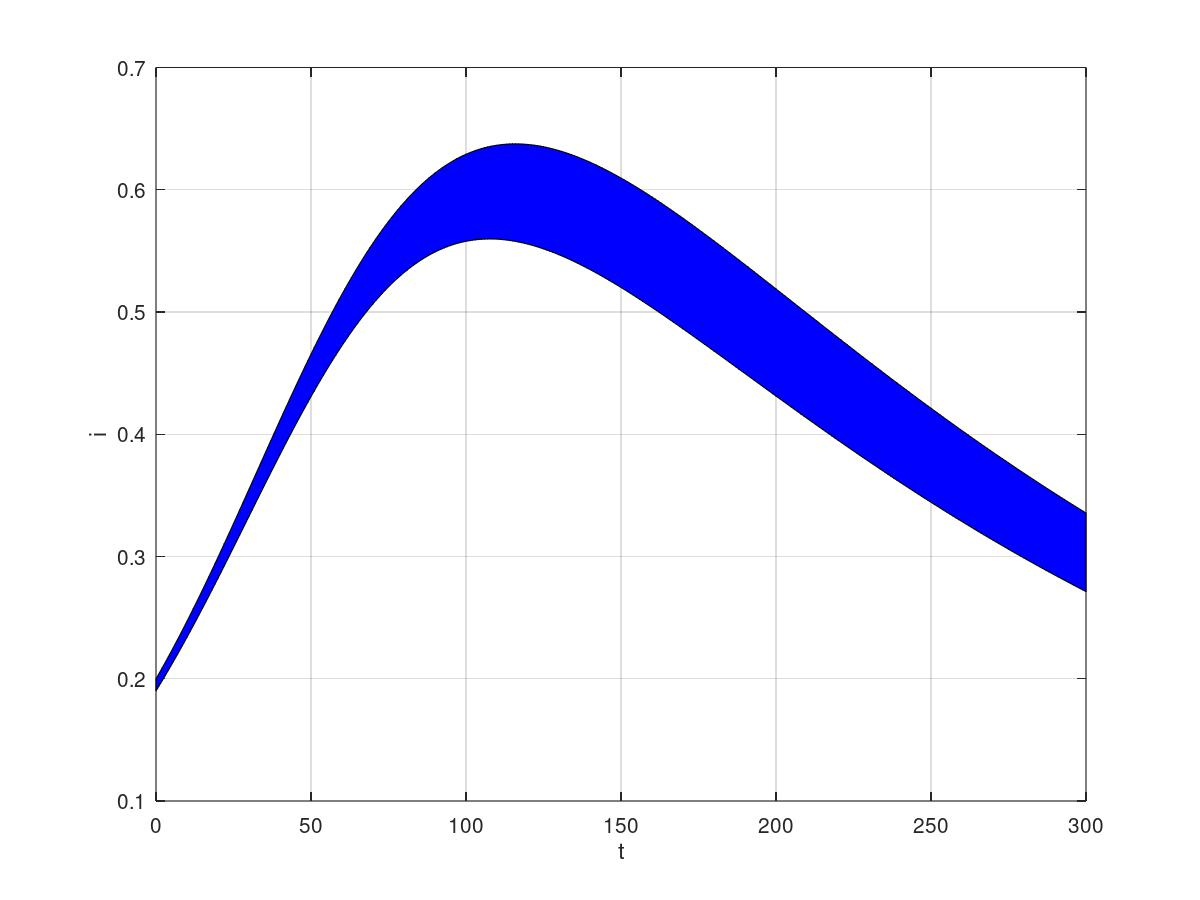
\includegraphics[width=\textwidth]{SapoFigures/SIR/SapoSIR_I.jpg}
    \end{subfigure}
    \begin{subfigure}{0.47\textwidth}
    \centering
    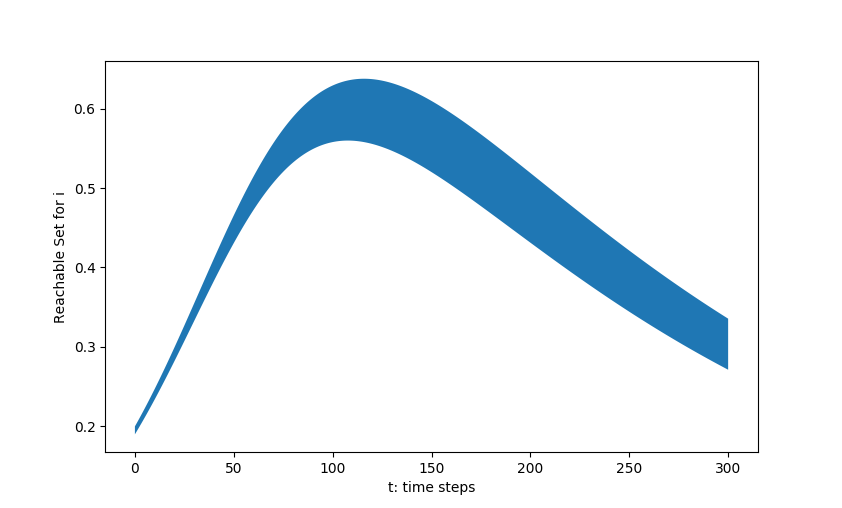
\includegraphics[width=1.2\textwidth,height=0.8\textwidth]{SapoFigures/SIR/KaaSIR_I.png}
    \end{subfigure}
  
%    \hspace{-15ex}  
    \begin{subfigure}{0.47\textwidth}
    \centering
    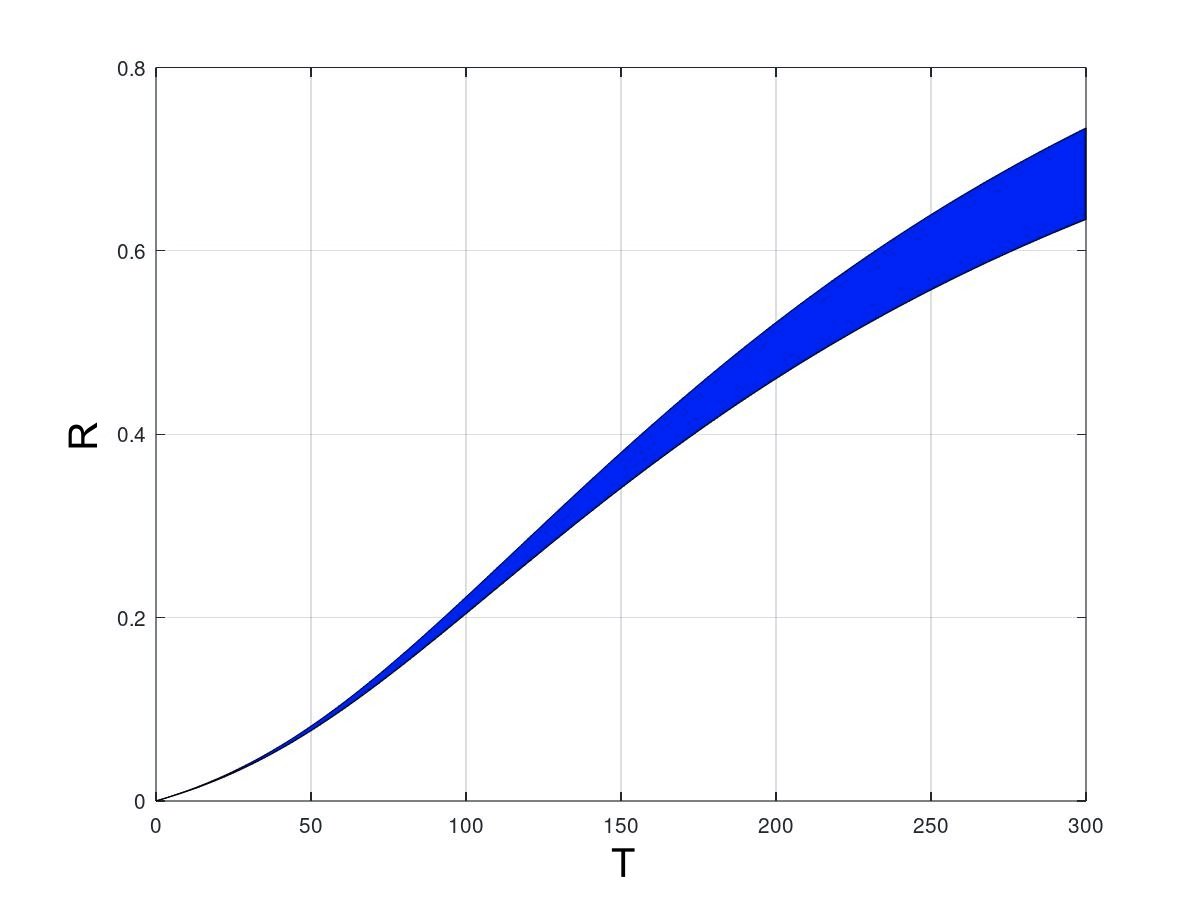
\includegraphics[width=\textwidth]{SapoFigures/SIR/SapoSIR_R.jpg}
    \end{subfigure}
    \begin{subfigure}{0.47\textwidth}
    \centering
    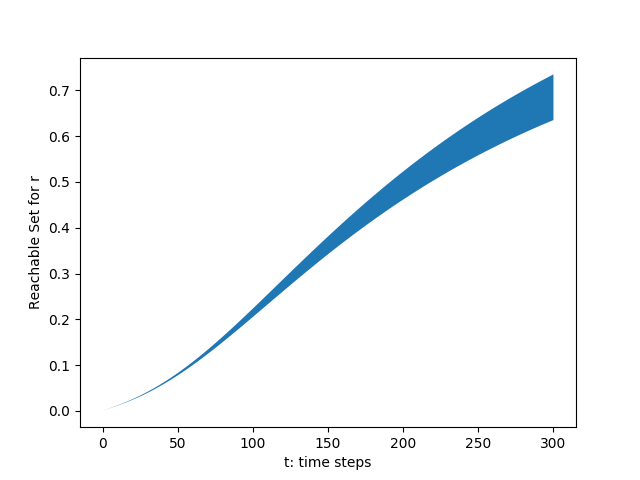
\includegraphics[width=1.2\textwidth]{SapoFigures/SIR/KaaSIR_R.png}
    \end{subfigure}
    
    \caption{Figure depicting the reachable set computation of the SIR model.} 
    \label{fig1}
\end{figure}

\begin{figure}[h]
%    \hspace{-15ex}
    \begin{subfigure}{0.47\textwidth}
    \centering
    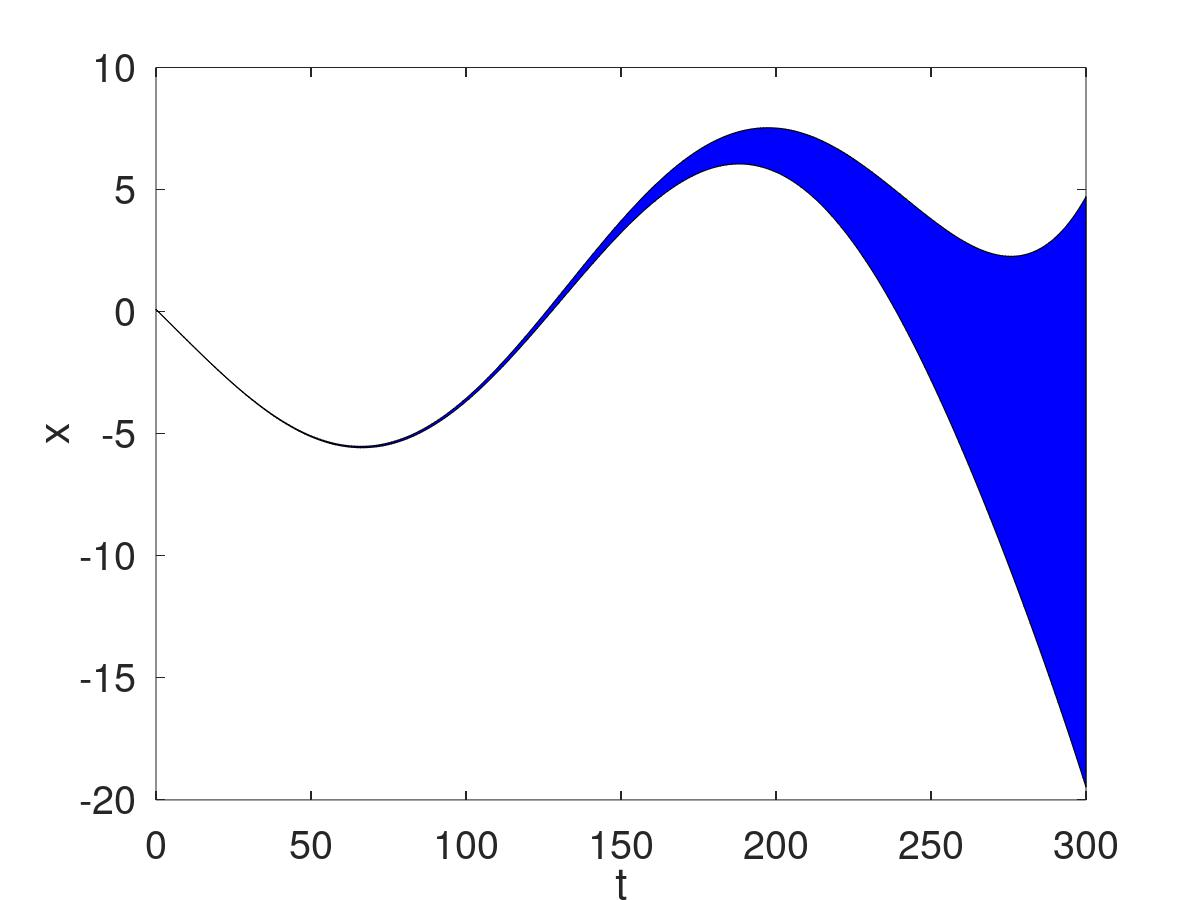
\includegraphics[width=\textwidth]{SapoFigures/Rosslert/SapoRossler_X.jpg}
    \end{subfigure}
    \begin{subfigure}{0.47\textwidth}
    \centering
    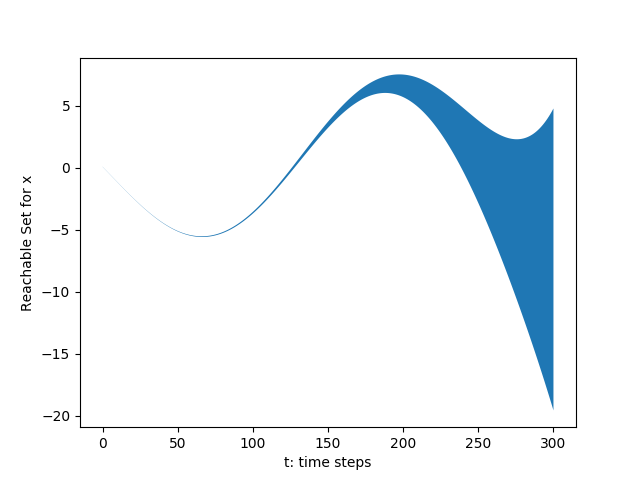
\includegraphics[width=1.3\textwidth]{SapoFigures/Rosslert/KaaRosslerX.png}
    \end{subfigure}
  
%     \hspace{-15ex}  
    \begin{subfigure}{0.47\textwidth}
    \centering
    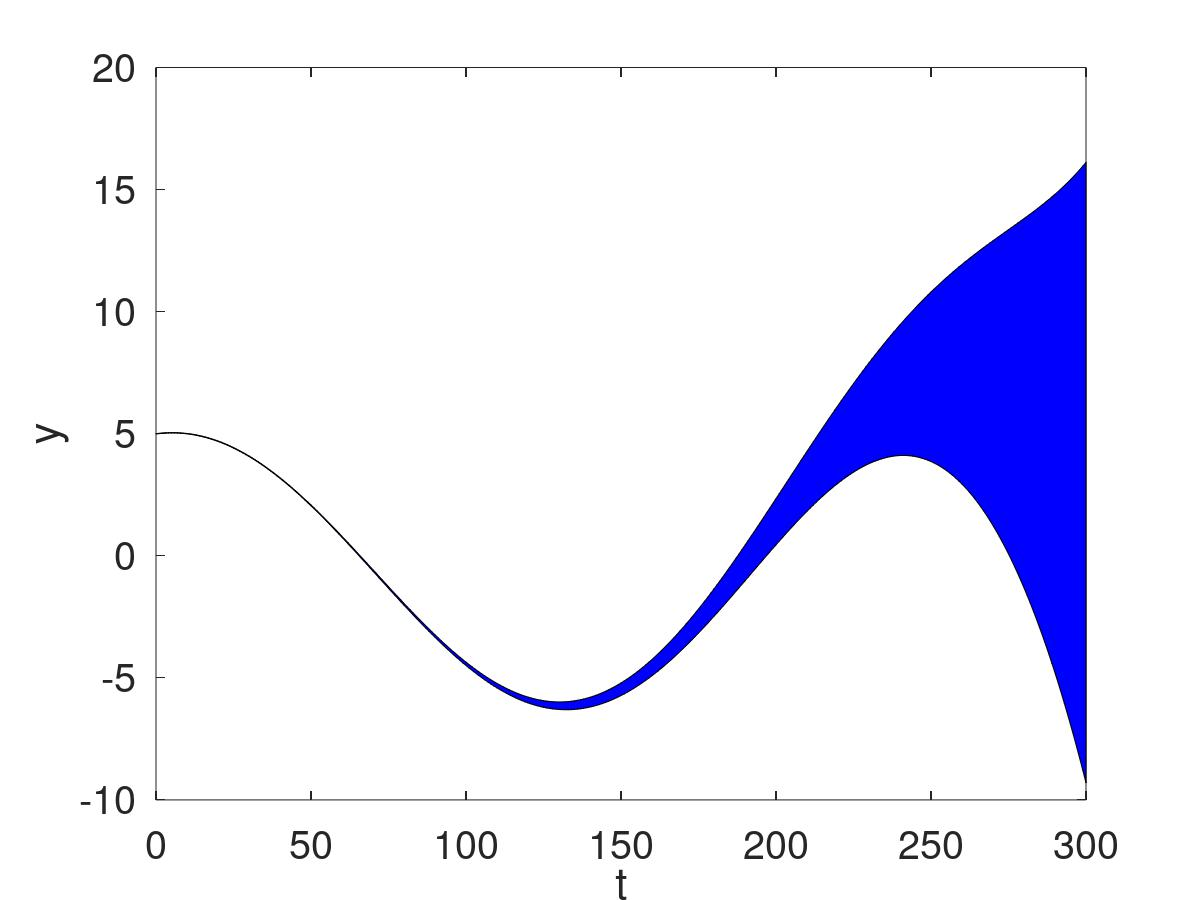
\includegraphics[width=\textwidth]{SapoFigures/Rosslert/SapoRossler_Y.jpg}
    \end{subfigure}
    % \hspace{-3ex}
    \begin{subfigure}{0.47\textwidth}
    \centering
    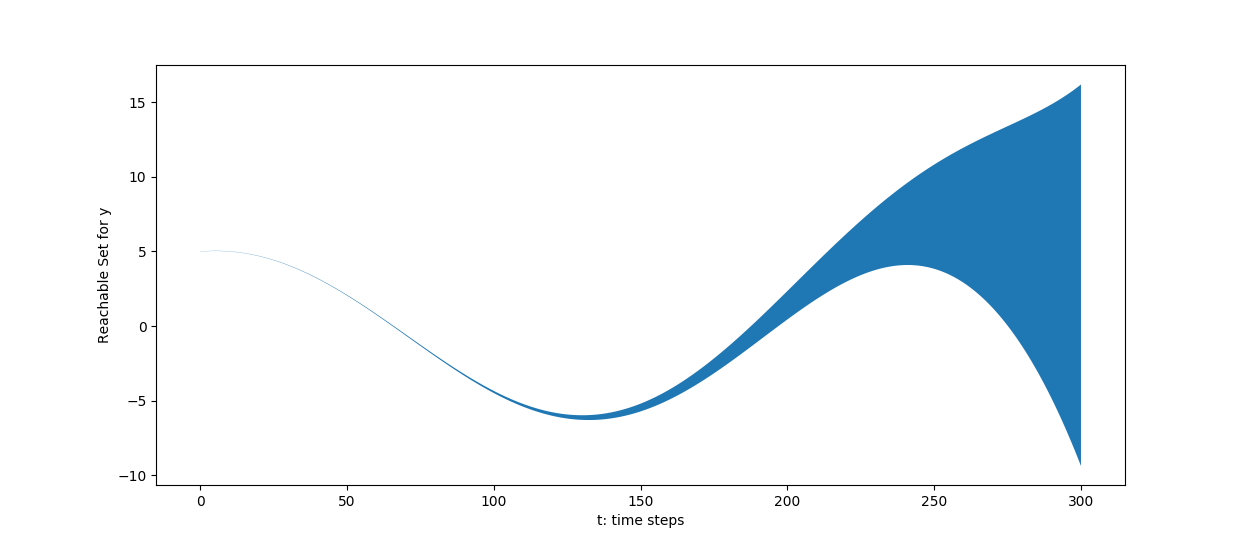
\includegraphics[width=1.3\textwidth,height=0.8\textwidth]{SapoFigures/Rosslert/KaaRosslerY.png}
    \end{subfigure}
  
%    \hspace{-15ex}  
    \begin{subfigure}{0.47\textwidth}
    \centering
    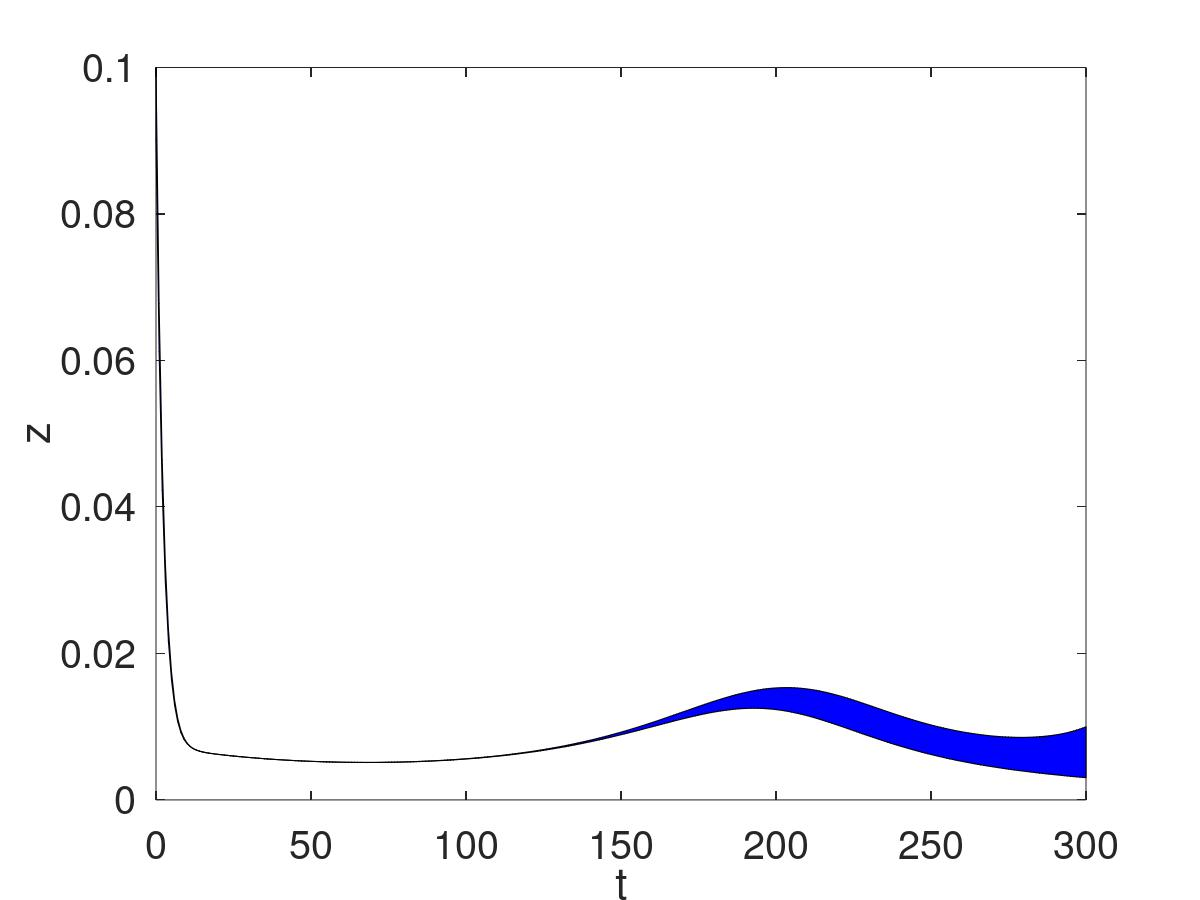
\includegraphics[width=\textwidth]{SapoFigures/Rosslert/SapoRossler_Z.jpg}
    \end{subfigure}
    \begin{subfigure}{0.47\textwidth}
    \centering
    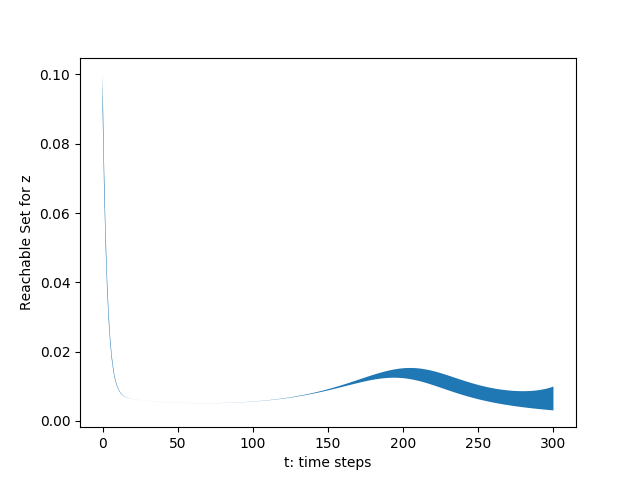
\includegraphics[width=1.3\textwidth]{SapoFigures/Rosslert/KaaRosslerZ.png}
    \end{subfigure}
    
    \caption{Figure depicting the reachable set computation of the Rossler model.} 
    \label{fig2}
\end{figure}    

\begin{figure}[h]
%    \hspace{-12ex}
    \begin{subfigure}{0.45\textwidth}
    \centering
    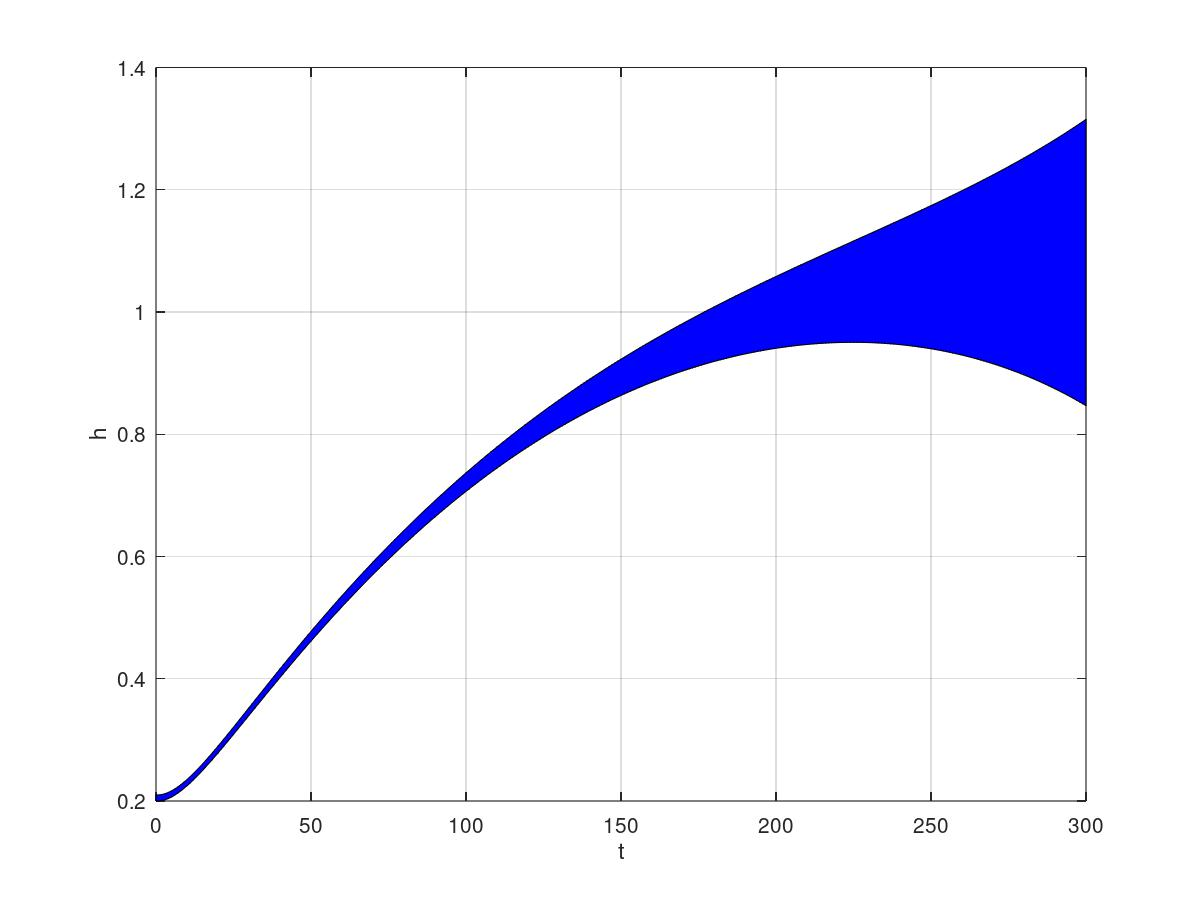
\includegraphics[width=\textwidth]{SapoFigures/Quad/SapoQuad_H.jpg}
    \end{subfigure}
    \begin{subfigure}{0.47\textwidth}
    \centering
    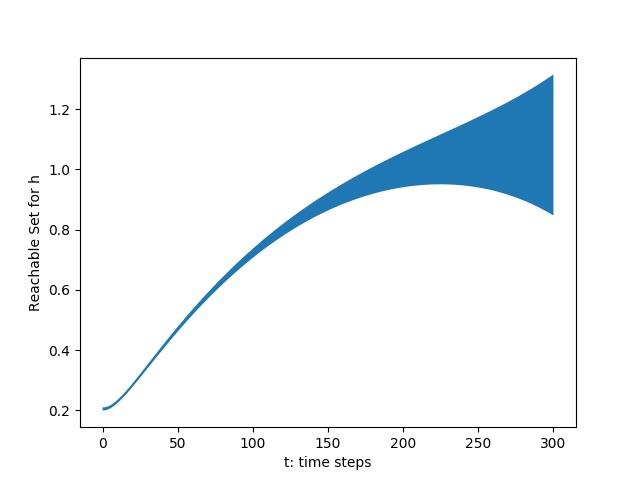
\includegraphics[width=1.1\textwidth,height=0.8\textwidth]{SapoFigures/Quad/KaaQuad_H.jpg}
    \end{subfigure}
    
%     \hspace{-12ex}
    \begin{subfigure}{0.45\textwidth}
    \centering
    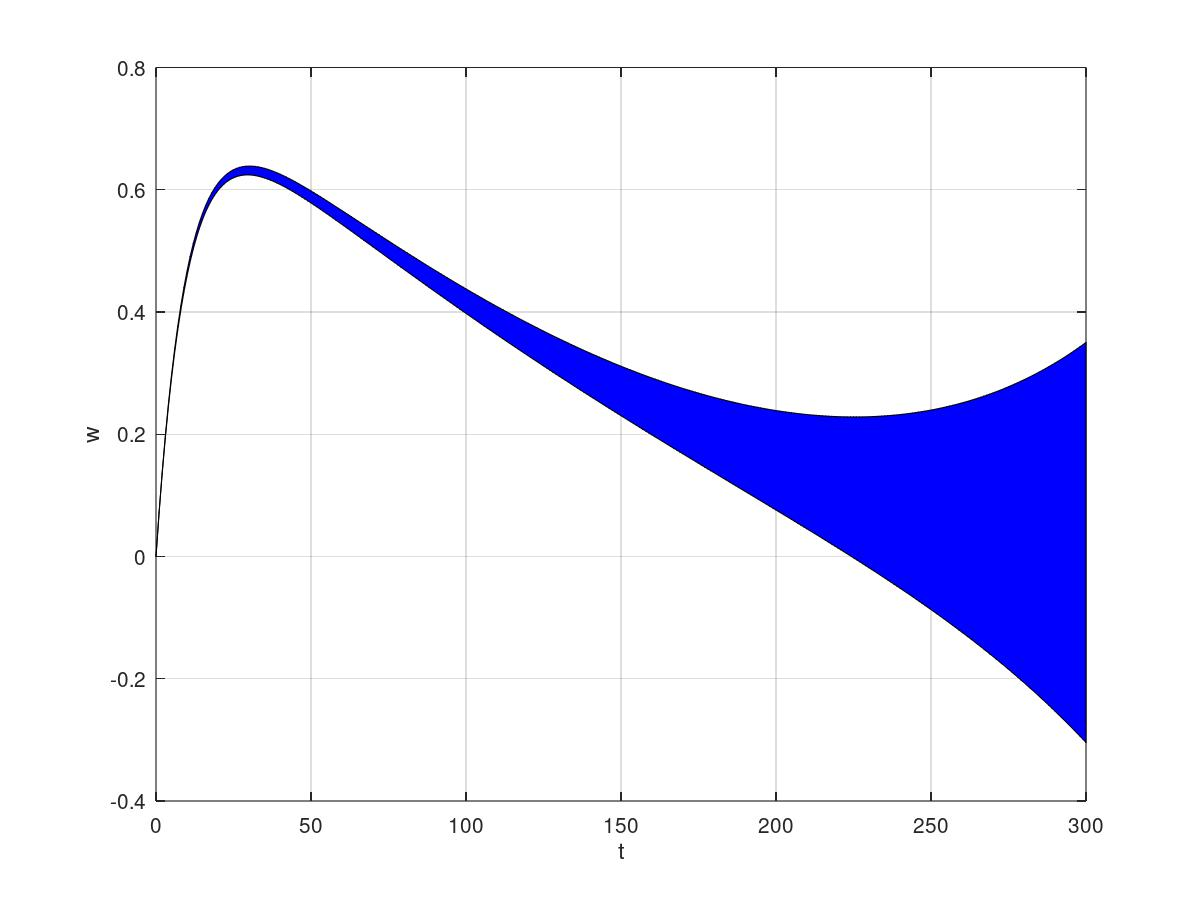
\includegraphics[width=\textwidth]{SapoFigures/Quad/SapoQuad_W.jpg}
    \end{subfigure}
    \begin{subfigure}{0.47\textwidth}
    \centering
    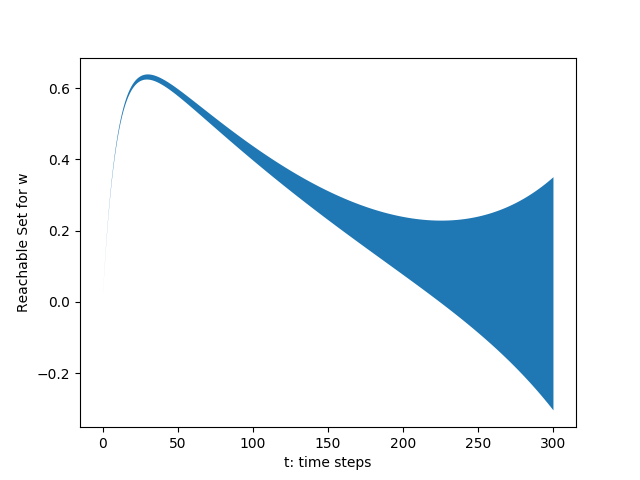
\includegraphics[width=1.1\textwidth,height=0.8\textwidth]{SapoFigures/Quad/KaaQuad_W.png}
    \end{subfigure}
    
%    \hspace{-12ex}
    \begin{subfigure}{0.45\textwidth}
    \centering
    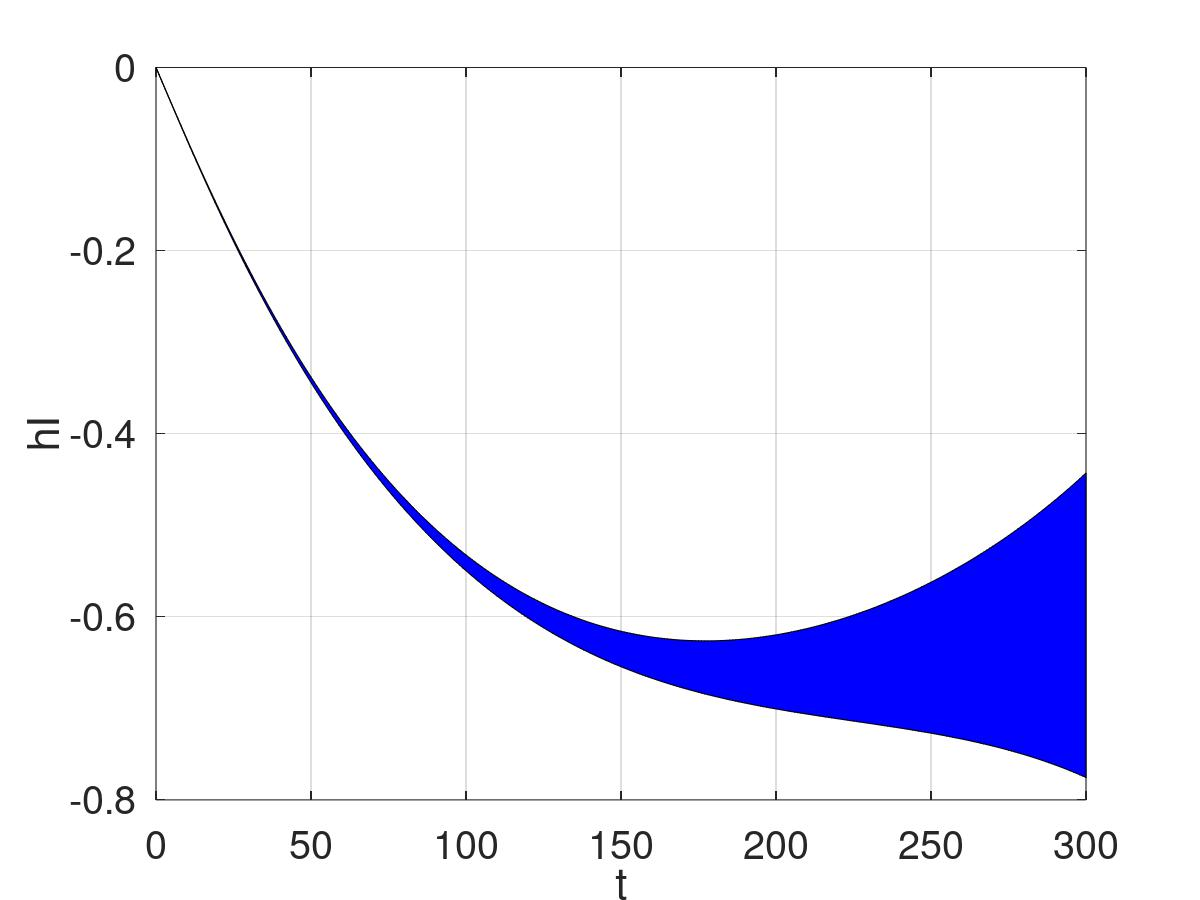
\includegraphics[width=\textwidth]{SapoFigures/Quad/SapoQuad_HI.jpg}
    \end{subfigure}
    \begin{subfigure}{0.47\textwidth}
    \centering
    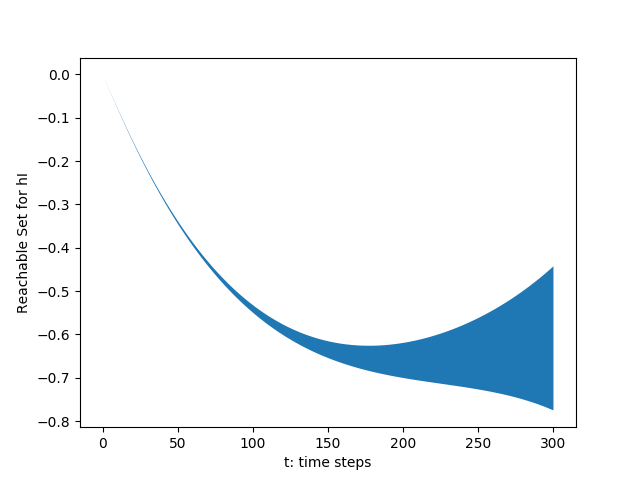
\includegraphics[width=1.1\textwidth,height=0.85\textwidth]{SapoFigures/Quad/KaaQuad_HI.png}
    \end{subfigure}
    
    \caption{Figure depicting the reachable set computation of the Quadcopter model.} 
    \label{fig3}
\end{figure}


\begin{figure}[h]
%    \hspace{-12ex}
    \begin{subfigure}{0.47\textwidth}
    \centering
    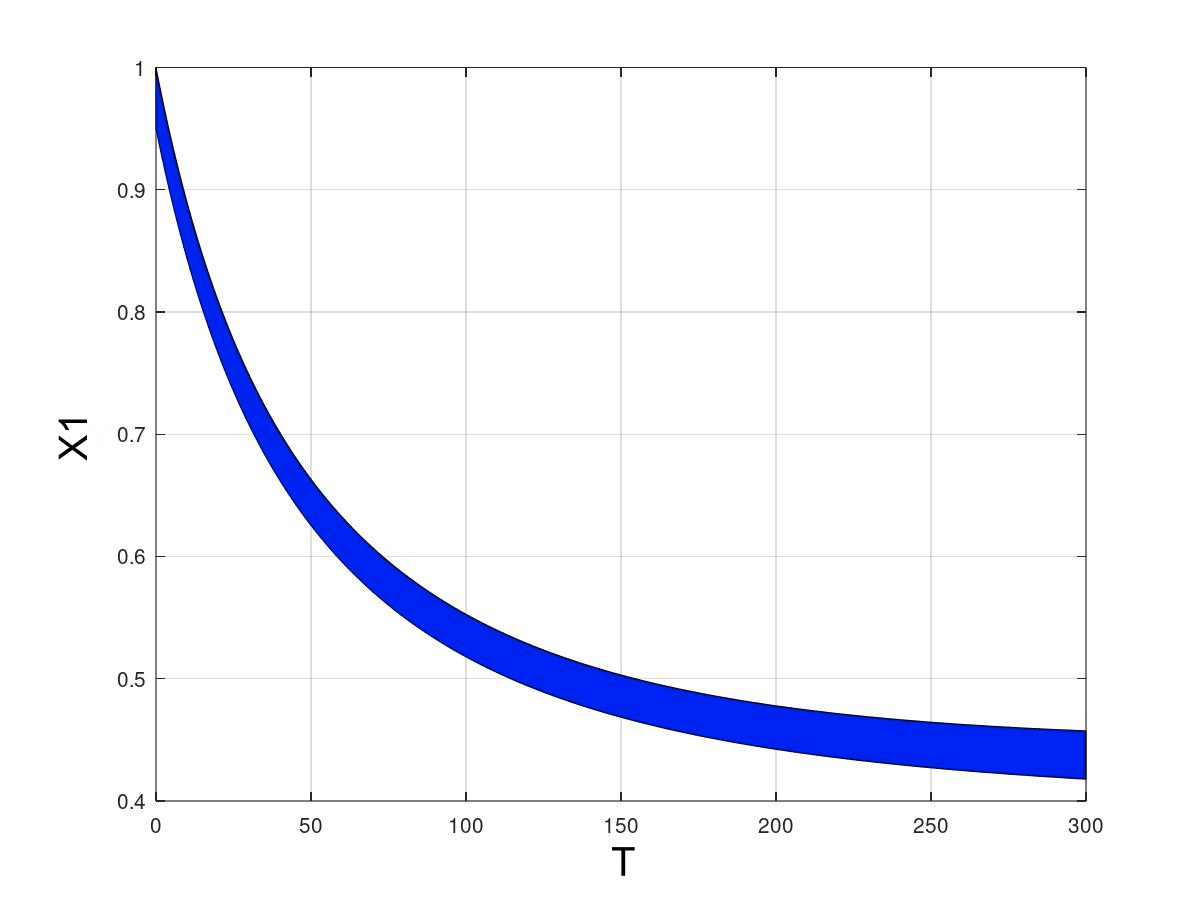
\includegraphics[width=\textwidth]{SapoFigures/LV/SapoLV_X1.jpg}
    \end{subfigure}
    \begin{subfigure}{0.47\textwidth}
    \centering
    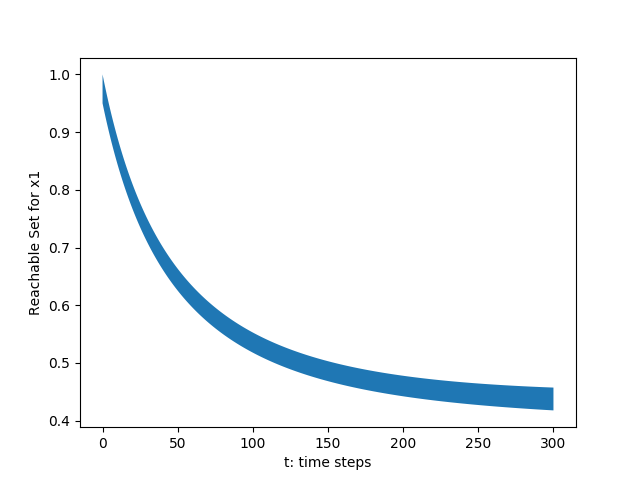
\includegraphics[width=1.1\textwidth,height=0.85\textwidth]{SapoFigures/LV/KaaLV_X1.png}
    \end{subfigure}
    
%     \hspace{-12ex}
    \begin{subfigure}{0.47\textwidth}
    \centering
    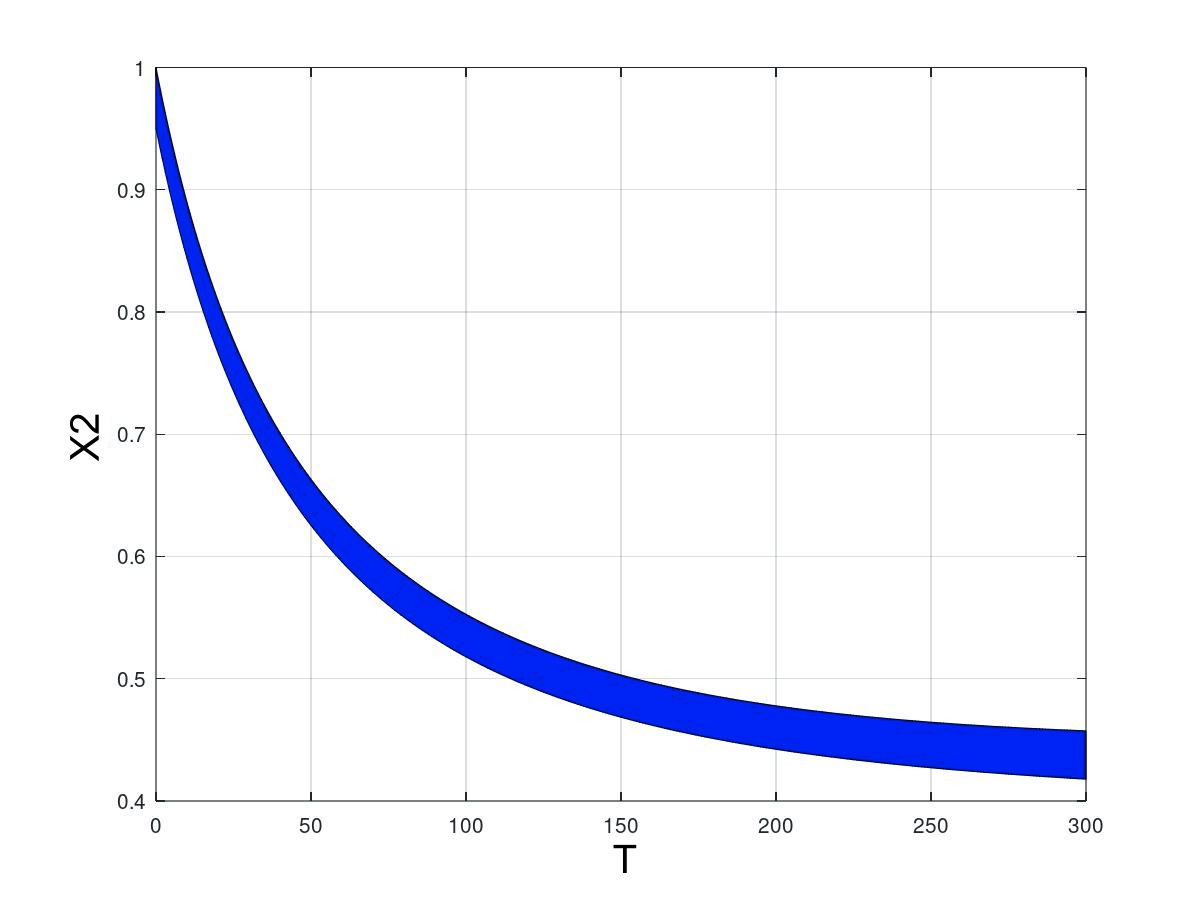
\includegraphics[width=\textwidth]{SapoFigures/LV/SapoLV_X2.jpg}
    \end{subfigure}
    \begin{subfigure}{0.47\textwidth}
    \centering
    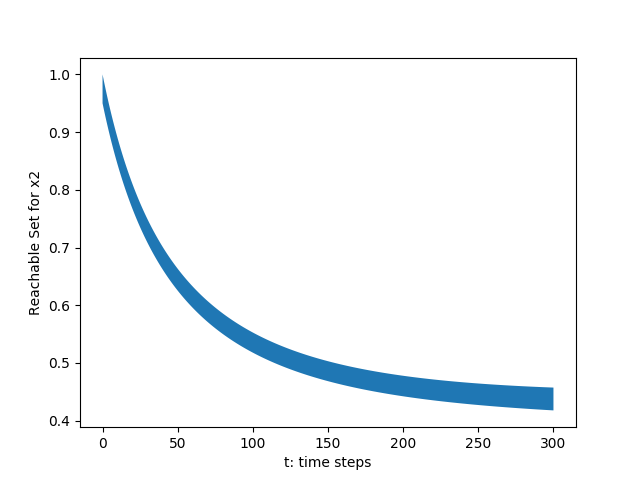
\includegraphics[width=1.1\textwidth,height=0.82\textwidth]{SapoFigures/LV/KaaLV_X2.png}
    \end{subfigure}
    
%    \hspace{-12ex}
    \begin{subfigure}{0.47\textwidth}
    \centering
    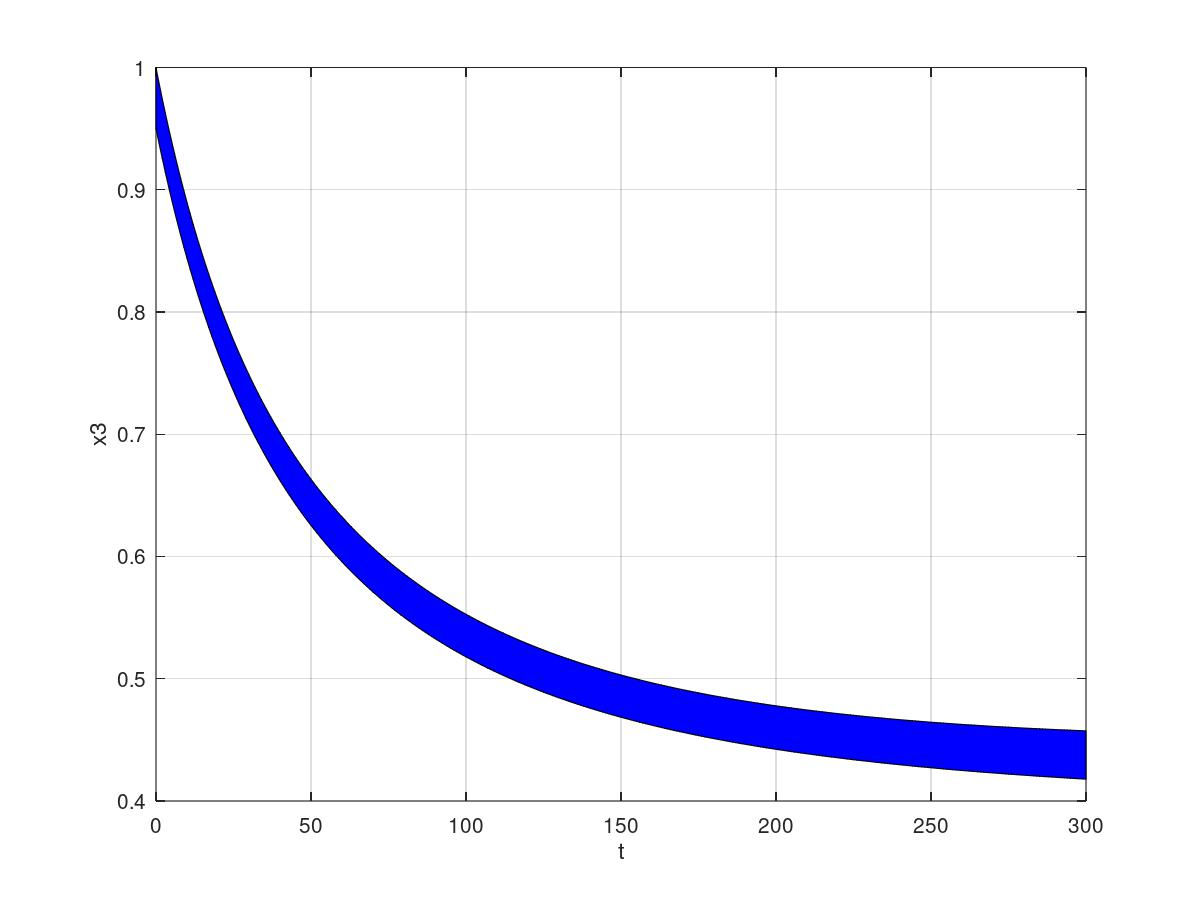
\includegraphics[width=\textwidth]{SapoFigures/LV/SapoLV_X3.jpg}
    \end{subfigure}
    \begin{subfigure}{0.47\textwidth}
    \centering
    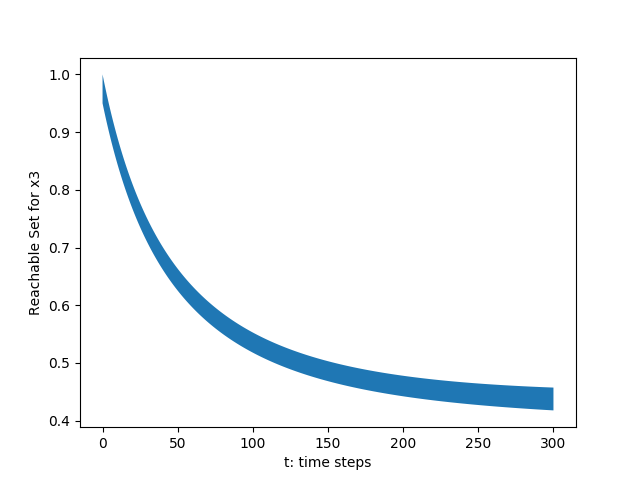
\includegraphics[width=1.1\textwidth,height=0.82\textwidth]{SapoFigures/LV/KaaLV_X3.png}
    \end{subfigure}
    
    \caption{Figure depicting the reachable set computation of the Lotka-Volterra model.} 
    \label{fig4}
\end{figure}

\begin{figure}[h]
%    \hspace{-12ex}
    \begin{subfigure}{0.47\textwidth}
    \centering
    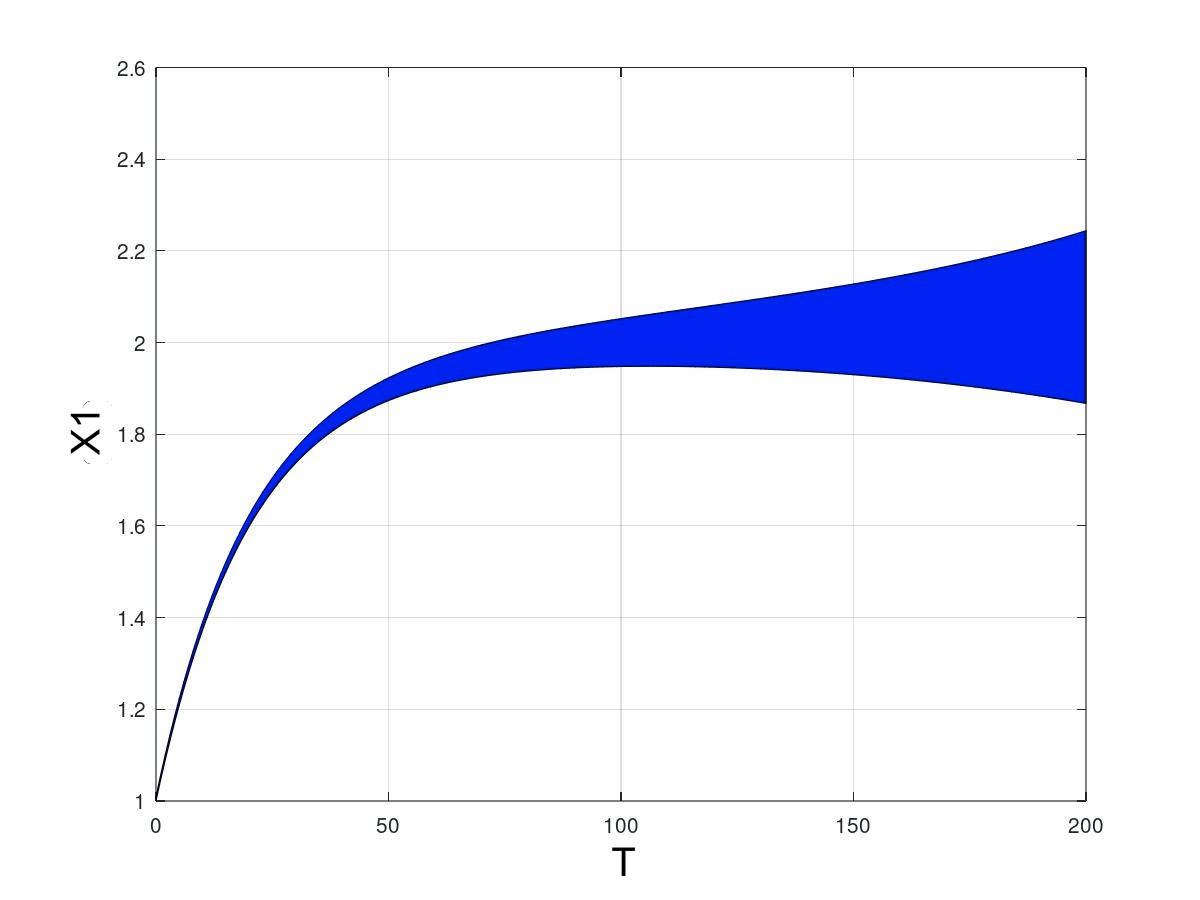
\includegraphics[width=\textwidth]{SapoFigures/Phos/SapoKaa_X1.jpg}
    \end{subfigure}
    \begin{subfigure}{0.47\textwidth}
    \centering
    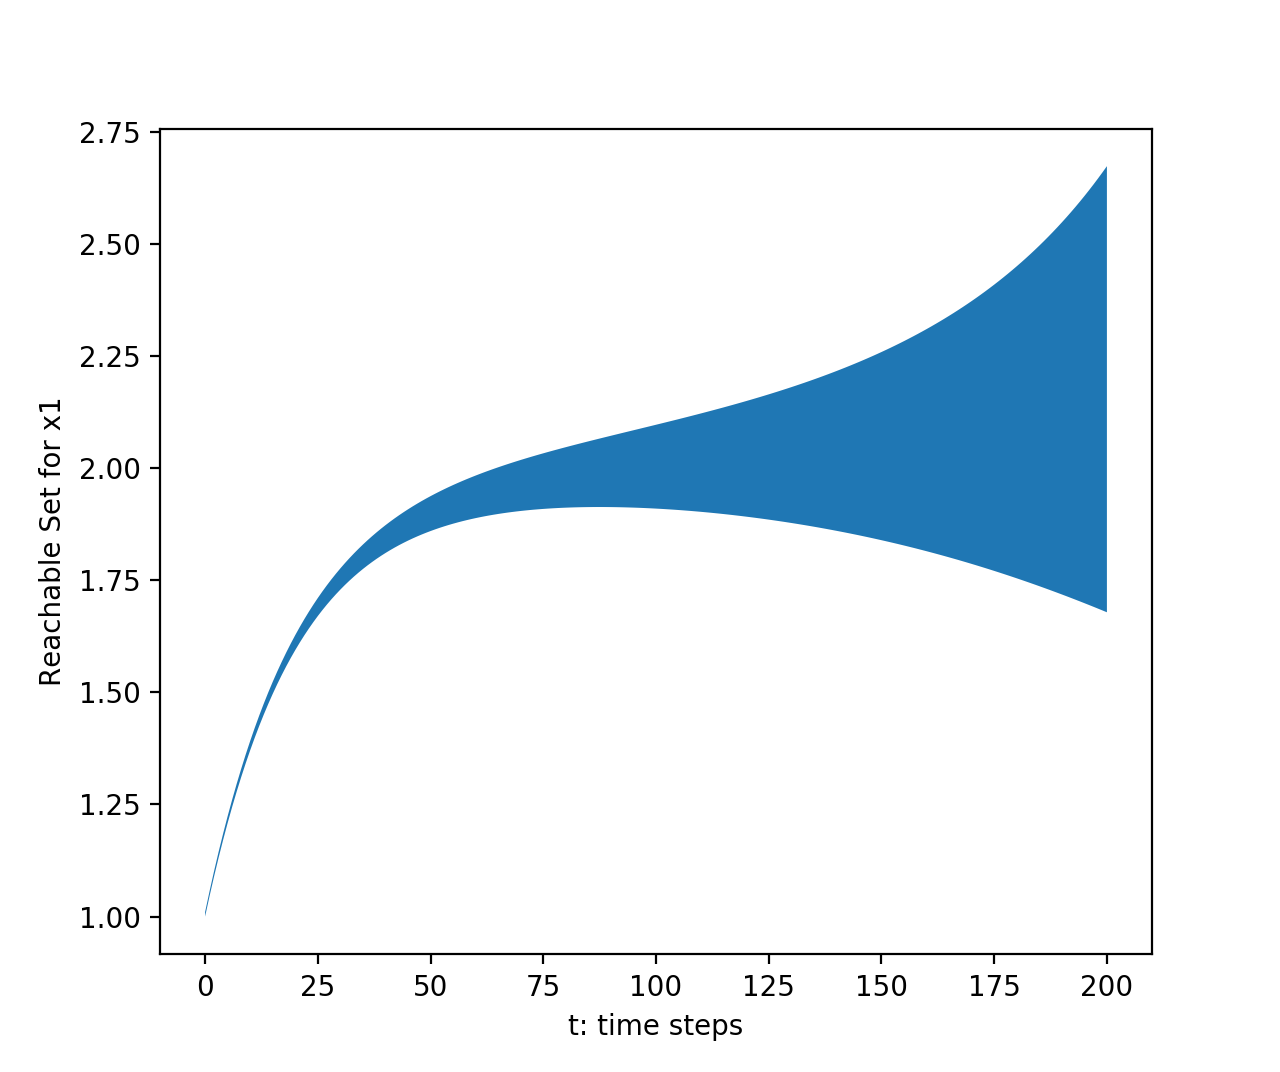
\includegraphics[width=1.1\textwidth,height=0.82\textwidth]{SapoFigures/Phos/KaaPhos_X1.png}
    \end{subfigure}
    
%   \hspace{-12ex}
    \begin{subfigure}{0.47\textwidth}
    \centering
    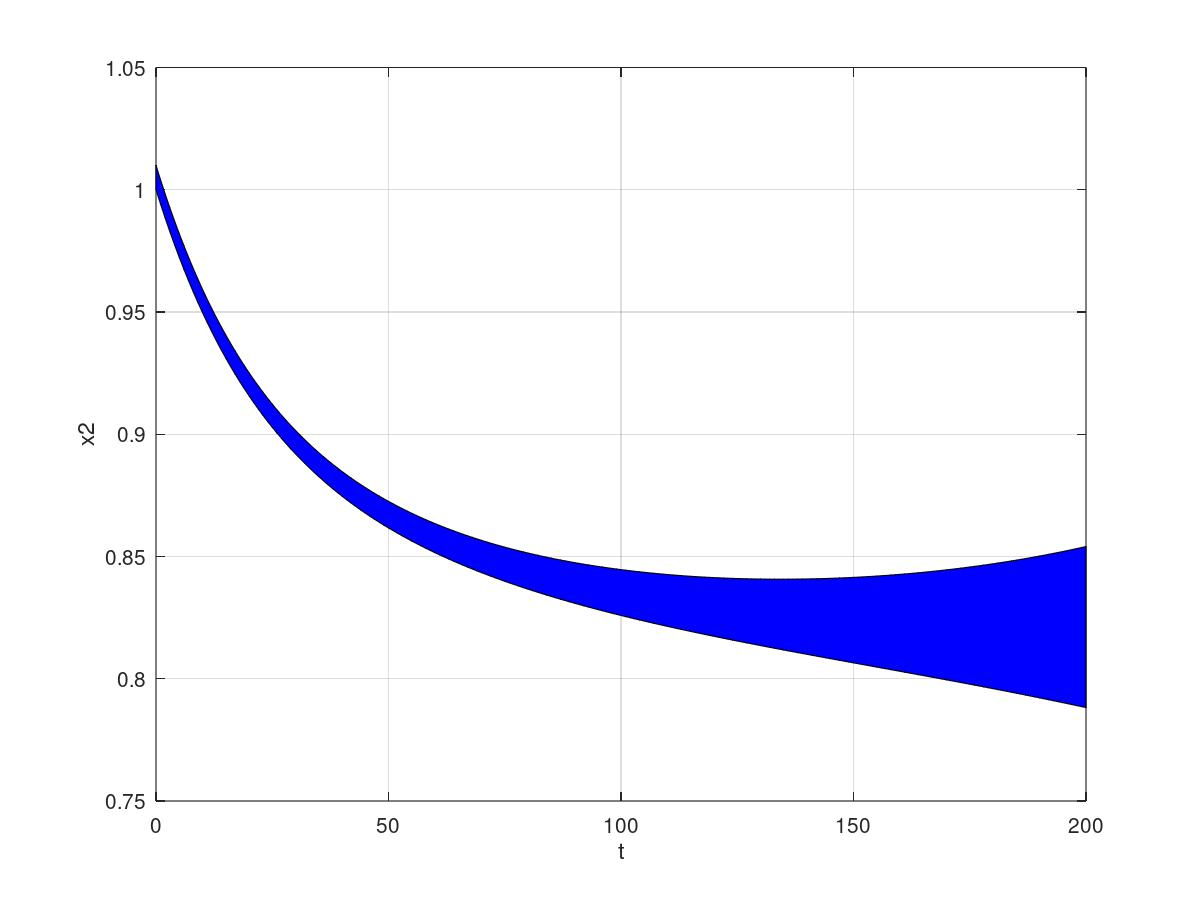
\includegraphics[width=\textwidth]{SapoFigures/Phos/SapoPhos_X2.jpg}
    \end{subfigure}
    \begin{subfigure}{0.47\textwidth}
    \centering
    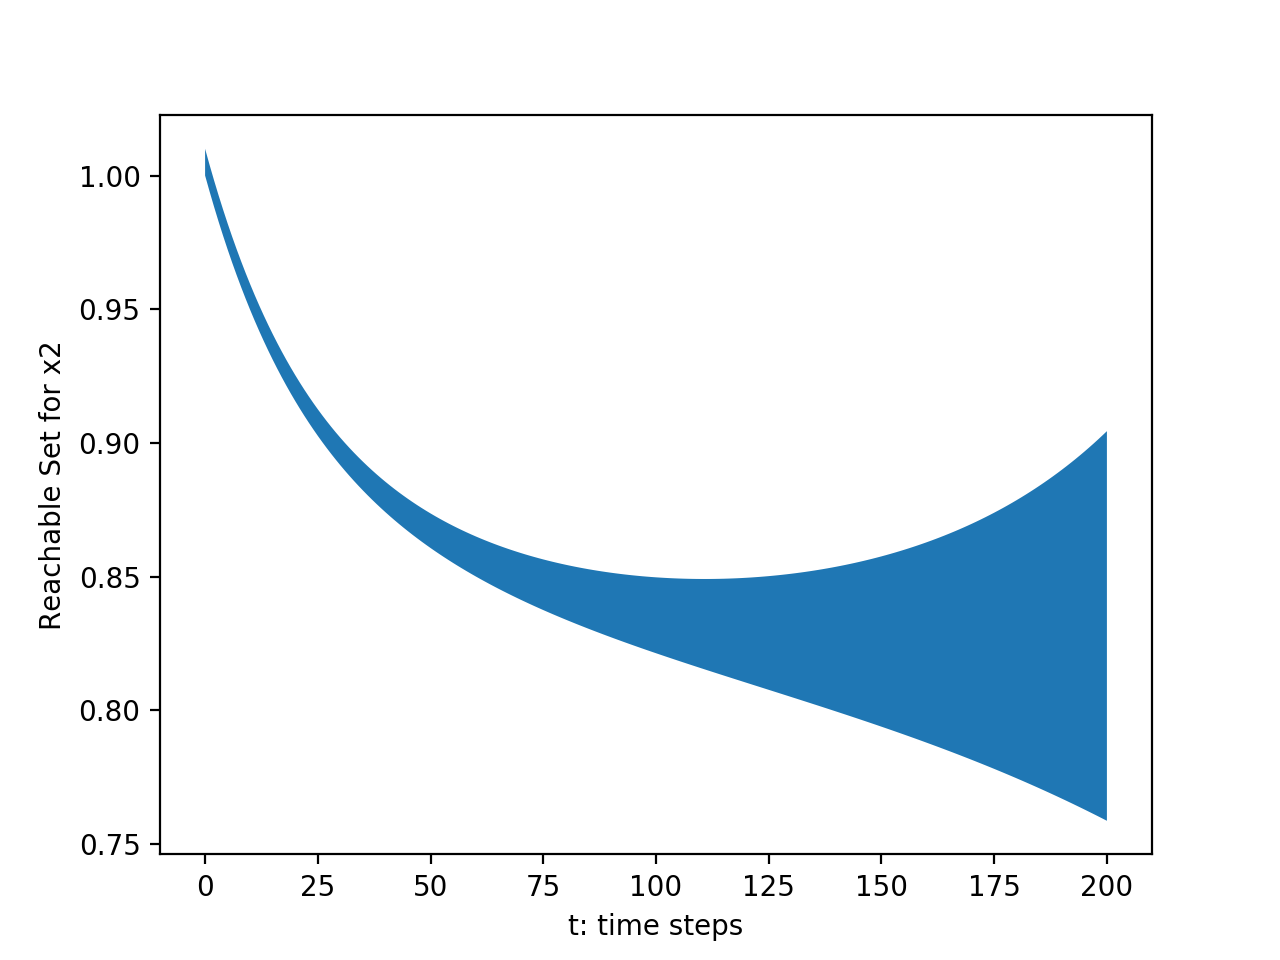
\includegraphics[width=1.1\textwidth,height=0.82\textwidth]{SapoFigures/Phos/KaaPhos_X2.png}
    \end{subfigure}
    
%   \hspace{-12ex}
    \begin{subfigure}{0.47\textwidth}
    \centering
    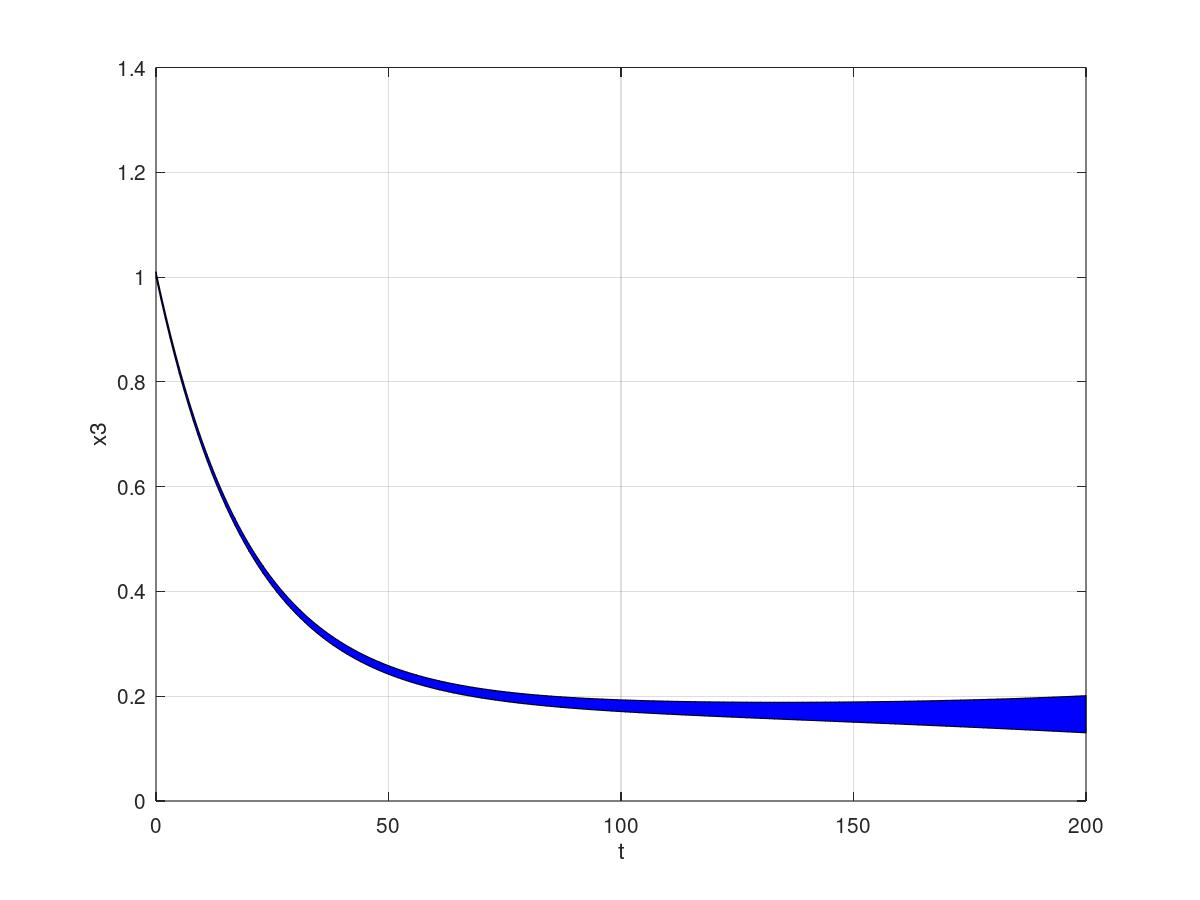
\includegraphics[width=\textwidth]{SapoFigures/Phos/SapoPhos_X3.jpg}
    \end{subfigure}
    \begin{subfigure}{0.47\textwidth}
    \centering
    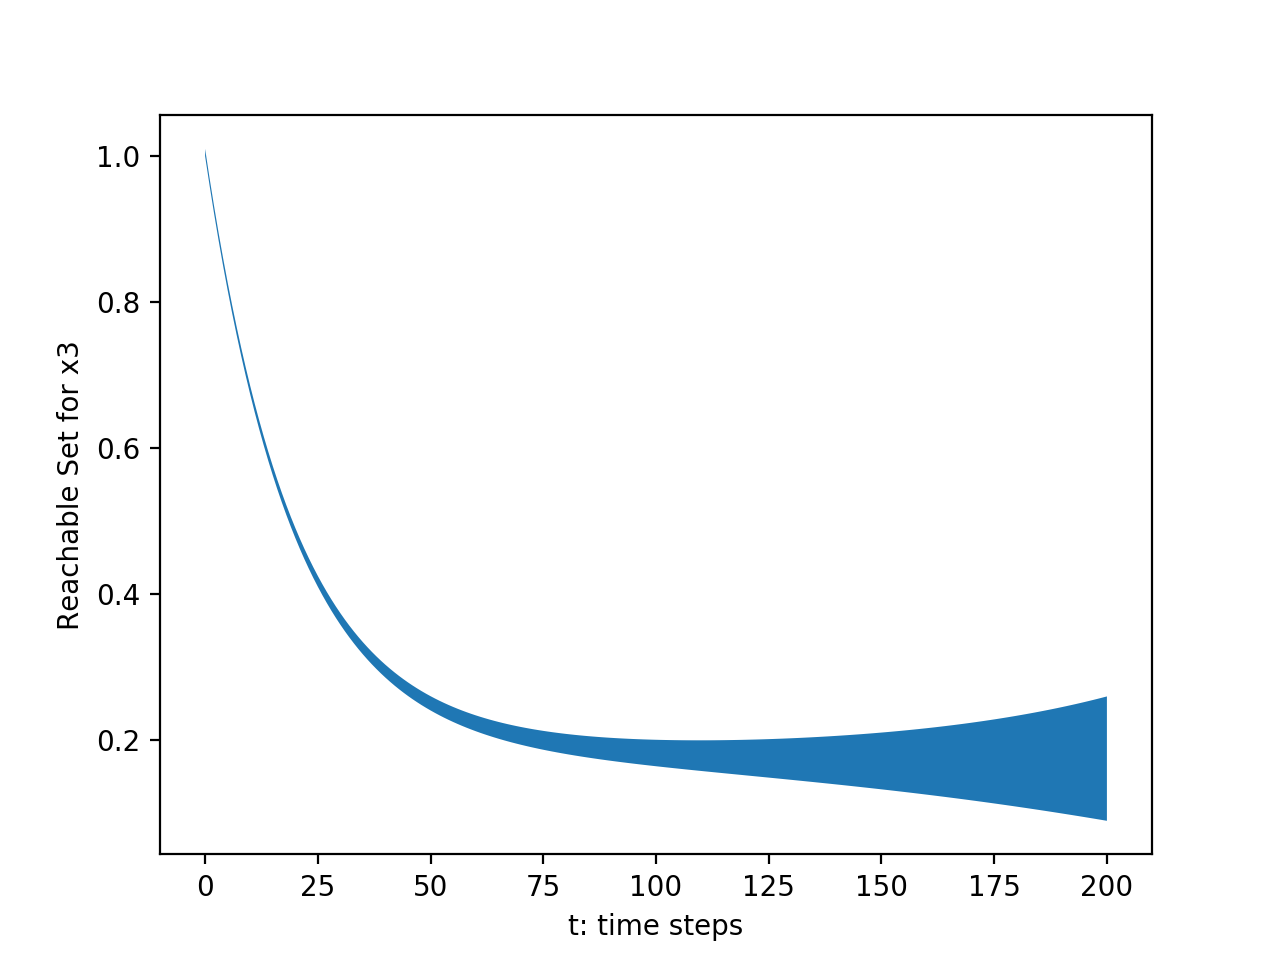
\includegraphics[width=1.1\textwidth,height=0.82\textwidth]{SapoFigures/Phos/KaaPhos_X3.png}
    \end{subfigure}
    
    \caption{Figure depicting the reachable set computation of the Phosporaley model.} 
    \label{fig5}
\end{figure}


% \begin{figure}
% 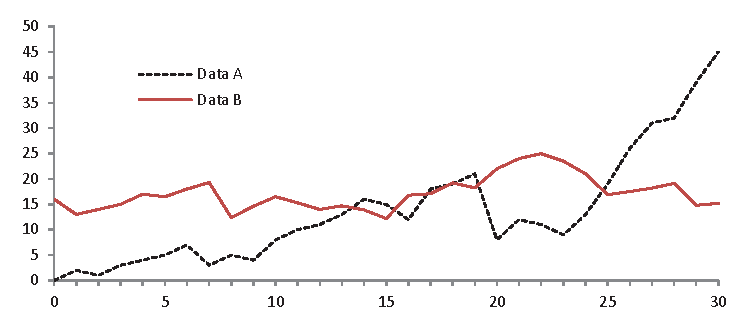
\includegraphics[width=\textwidth]{Figures/fig1.eps}
% \caption{A figure caption is always placed below the illustration.
% Please note that short captions are centered, while long ones are
% justified by the macro package automatically.} \label{fig1}
% \end{figure}


% For citations of references, we prefer the use of square brackets
% and consecutive numbers. Citations using labels or the author/year
% convention are also acceptable. The following bibliography provides
% a sample reference list with entries for journal
% articles~\cite{ref_article1}, an LNCS chapter~\cite{ref_lncs1}, a
% book~\cite{ref_book1}, proceedings without editors~\cite{ref_proc1},
% and a homepage~\cite{ref_url1}. Multiple citations are grouped
% \cite{ref_article1,ref_lncs1,ref_book1},
% \cite{ref_article1,ref_book1,ref_proc1,ref_url1}.
%
% ---- Bibliography ----
%
% BibTeX users should specify bibliography style 'splncs04'.
% References will then be sorted and formatted in the correct style.
%

%
% \begin{thebibliography}{8}
% \bibitem{ref_article1}
% Author, F.: Article title. Journal \textbf{2}(5), 99--110 (2016)

% \bibitem{ref_lncs1}
% Author, F., Author, S.: Title of a proceedings paper. In: Editor,
% F., Editor, S. (eds.) CONFERENCE 2016, LNCS, vol. 9999, pp. 1--13.
% Springer, Heidelberg (2016). \doi{10.10007/1234567890}

% \bibitem{ref_book1}
% Author, F., Author, S., Author, T.: Book title. 2nd edn. Publisher,
% Location (1999)

% \bibitem{ref_proc1}
% Author, A.-B.: Contribution title. In: 9th International Proceedings
% on Proceedings, pp. 1--2. Publisher, Location (2010)

% \bibitem{ref_url1}
% LNCS Homepage, \url{http://www.springer.com/lncs}. Last accessed 4
% Oct 2017
% \end{thebibliography}
\end{document}
